%In this chapter I introduce the \gls{NOvA} Test Beam experiment in Sec.~\ref{sec:TBExperiment}, focusing on the Test Beam detector and especially on the aspects that could impact its calibration. Section~\ref{sec:DataBasedSimulation} describes the new data-based simulation of cosmic muons that I developed for the Test Beam detector calibration, while Sec.~\ref{sec:TBCalibrationSection} discusses the calibration of the Test Beam detector itself.

\chapter{Data-based simulation of cosmic muons}\label{sec:DataBasedSimulation}

The standard \gls{NOvA} calibration procedure described in Sec.~\ref{sec:NOvACalibration} uses the \gls{CRY} \gls{MC} generator (see Sec.~\ref{sec:NOvASimulation}) to create the simulated cosmic ray sample for calibration. However, \gls{CRY} proved to be inefficient, generating particles failing to hit the detector, resulting in wasted processing resources and disk space. Moreover, the momentum and angle distributions in \gls{CRY} are not well suited to the \gls{NOvA} sites, potentially impacting the calibration accuracy.

To overcome these challenges, I developed and implemented a data-based simulation that eliminates the need for the \gls{CRY} \gls{MC} generator. Instead, I use a subset of the cosmic data sample used in calibration, pulling information on the muon vertex position, direction and momentum, to use, after some corrections and smearing, as inputs to the detector simulation to create a new simulated cosmic ray sample.

This approach results in a near-perfect efficiency, ensuring that almost every simulated muon contributes to the final calibration sample, thus saving processing time, file size, and storage. Additionally, the simulated muon distributions are inherently consistent with the distributions from data. Given that the calibration chain itself is a time and computing intensive process, the reduction in the number of simulation files and in their sizes has significant benefits downstream of the file generation. 
%On the other hand, using real data to seed the simulation could introduce undesirable bias, if we do not carefully consider possible misreconstruction or selection bias.\note{Can I re-word the last sentence?}
%Using real world data introduces bias from known and unknown effects, such as varying detector efficiency or readout faults... We need to carefully consider and mitigate these effects when creating the simulation to make sure of its validity

In this chapter I introduce the new data-based simulation of cosmic muons that I developed for the Test Beam detector calibration. Section~\ref{sec:CosmicGenAna} introduces the reconstruction and selection of the data events used to create the simulation, Sec.~\ref{sec:DataBasedSimPython} mentions the corrections applied to this data to mitigate various reconstruction and selection effects, and Sec.~\ref{sec:DataBasedSimValidation} and \ref{sec:DataBasedSimSummary} discuss and summarise the simulation results.

\section{Reconstruction and selection of cosmic data events}\label{sec:CosmicGenAna}
It is important to choose a data sample that represents the detector in an ideal state, with as few known issues as possible. For Test Beam, we chose the period 4 data sample (see Tab.~\ref{tab:TestBeamPeriods}), as the other periods had complications such as faulty \glspl{FEB}, or underfilled cells. We only used half of period 4 data by skipping every other sub-run to limit the number of simulated events to that necessary for a successful calibration.

%Our goal is to examine the response of the \textbf{simulated detector} to realistic cosmic muons found in the \textbf{real data}. We therefore need to use well-reconstructed and selected cosmic muons from data to generate our simulation. If the selection of the reconstructed data does not accurately correspond to reality, either due to misreconstruction or incorrect selection criteria, it can introduce bias into our simulation.

We designed the reconstruction and selection criteria so that the majority of the simulated cosmic muons make it into the final simulation calibration sample. Therefore, we employed a similar process to that used to create the data calibration samples. Additionally, we require all distributions of the selected events to be well-understood and to resemble those of the data calibration samples.

\subsection*{Remove beam spills}
The first step is to remove beam spill events based on their time relative to the time of the beam spill. For Test Beam the beam spill is $\unit[4.2]{s}$ long and we remove all events within a $\unit[5]{s}$ window from the start of the beam spill, as shown in Fig.~\ref{fig:RemoveTBSpills}. This should leave us with mostly cosmic events.

\begin{figure}[hbtp]
\centering
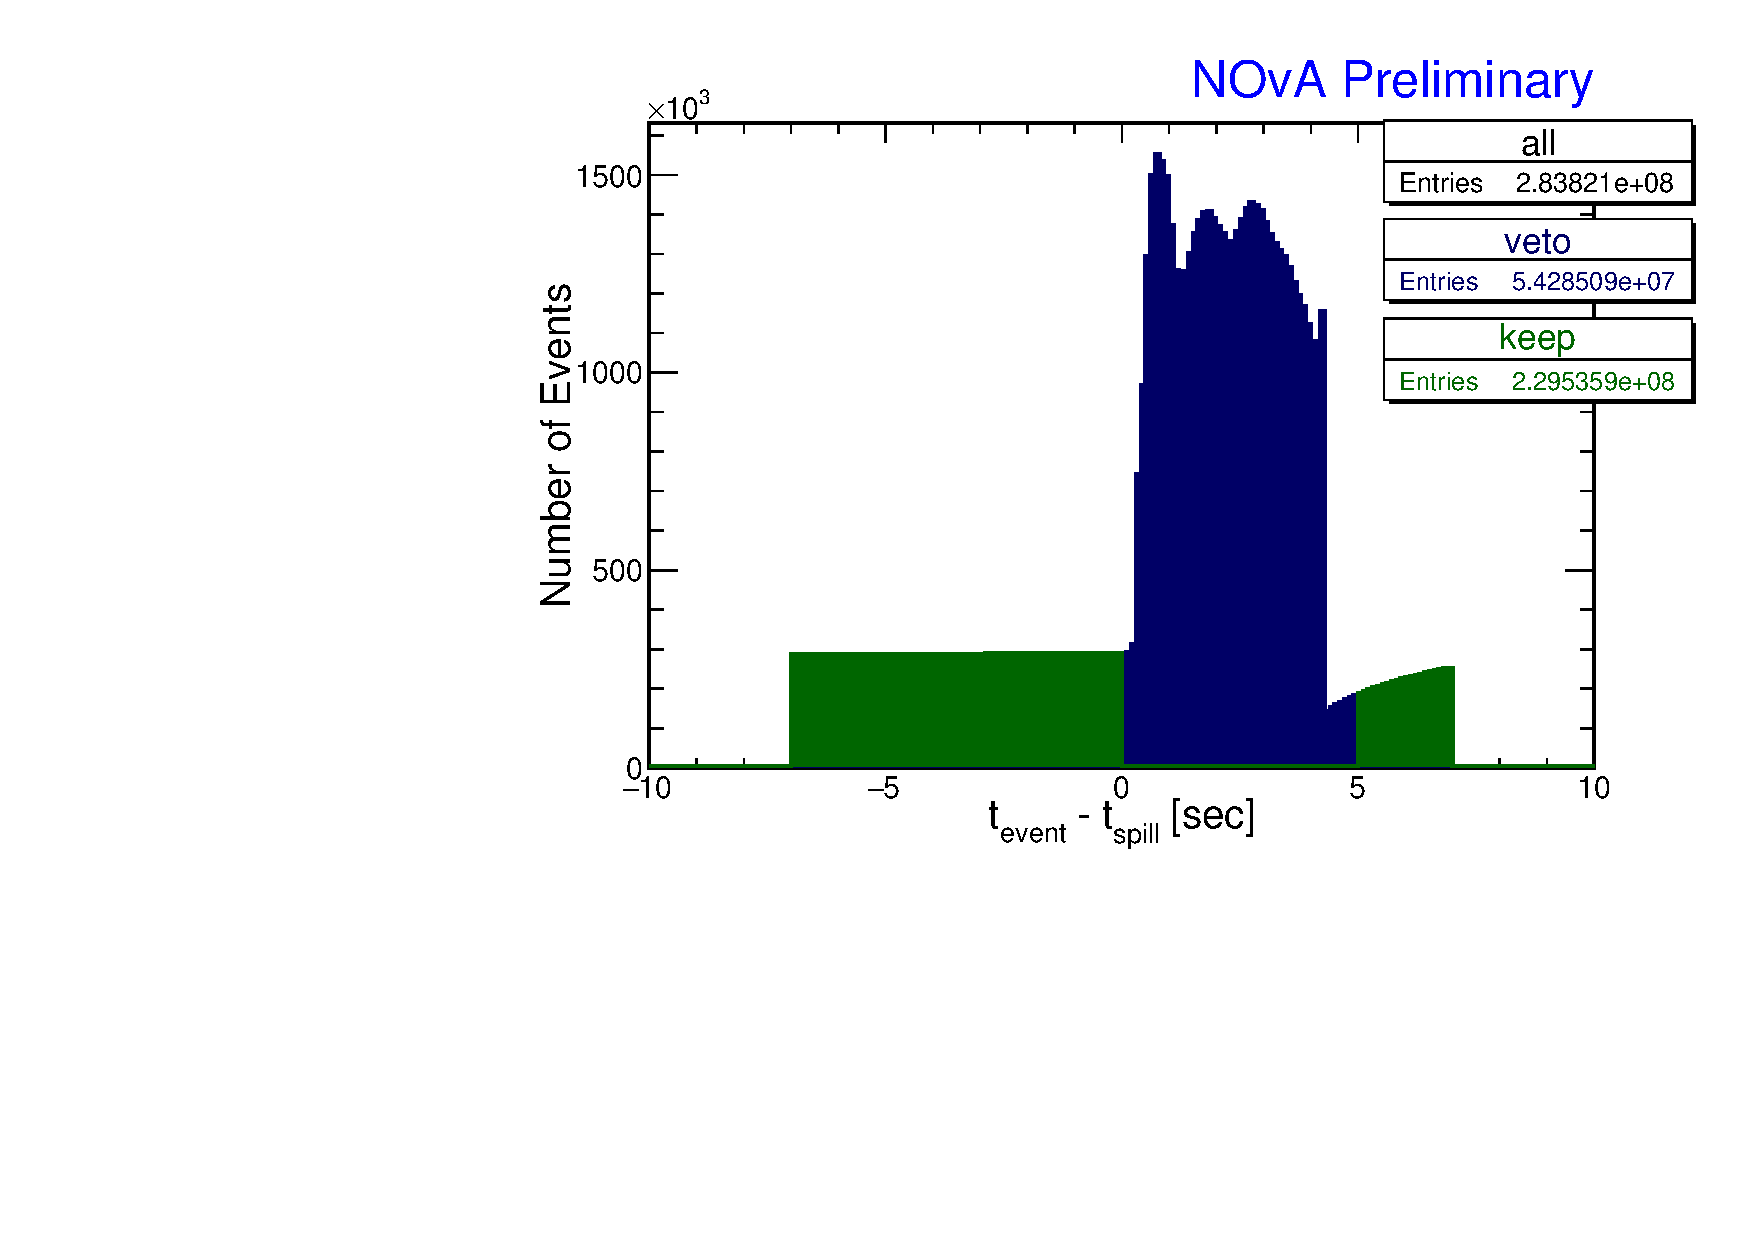
\includegraphics[width=\textwidth]{Plots/TBCalibration/RemoveTBSpills.pdf}
\caption[Removing Test Beam beam spill]{Test Beam beam spill events removed (blue) from the calibration samples. The remaining events (green) should mostly consist of cosmic particles. This example and the numbers of entries are for the full period 4 Test Beam sample.}
\label{fig:RemoveTBSpills}
\end{figure}

\subsection*{Reconstruction}
To use data events in simulation, we need to reconstruct their vertex positions and their initial 4-momenta. We use the standard reconstruction methods from \gls{NOvA}, described in Sec.~\ref{sec:NOvAReconstruction}. First we take the raw hits and group them into slices. Then we reconstruct cosmic tracks using the window cosmic track algorithm (used for calibration samples). Since we also require the 4-momentum information we have to use the \gls{BPF} tracking algorithm to identify muons and assign their momenta. \gls{BPF} requires vertex and prong input information, which we get from a cosmic ray vertex and FuzzyK prong algorithms respectively. The first three steps are identical to the full reconstruction applied to both data and simulation to produce the calibration samples. Since we do not need a 4-momentum information for calibration, we do not need to use cosmic ray vertex, FuzzyK vertex, or the \gls{BPF} to create calibration samples.

\subsection*{Selection}\label{sec:DataBasedSimSelection}
After the reconstruction process, we proceed to select events based on their slice and \gls{BPF} track properties. The overview of all selection criteria and their corresponding cut values are listed in Tab.~\ref{tab:DataBasedSimEventSelection}. In detail, the following conditions are used to select cosmic muon events for the data-based simulation:
\begin{enumerate}
\item We only use successfully reconstructed 3D \gls{BPF} tracks with the muon assumption;
\item As we aim to select cosmic events originating outside the detector, we apply a cut based on the distance of each track's start position from the edges of the detector. This cut has a negligible impact on the \gls{BPF} tracks;

\begin{figure}[!ht]
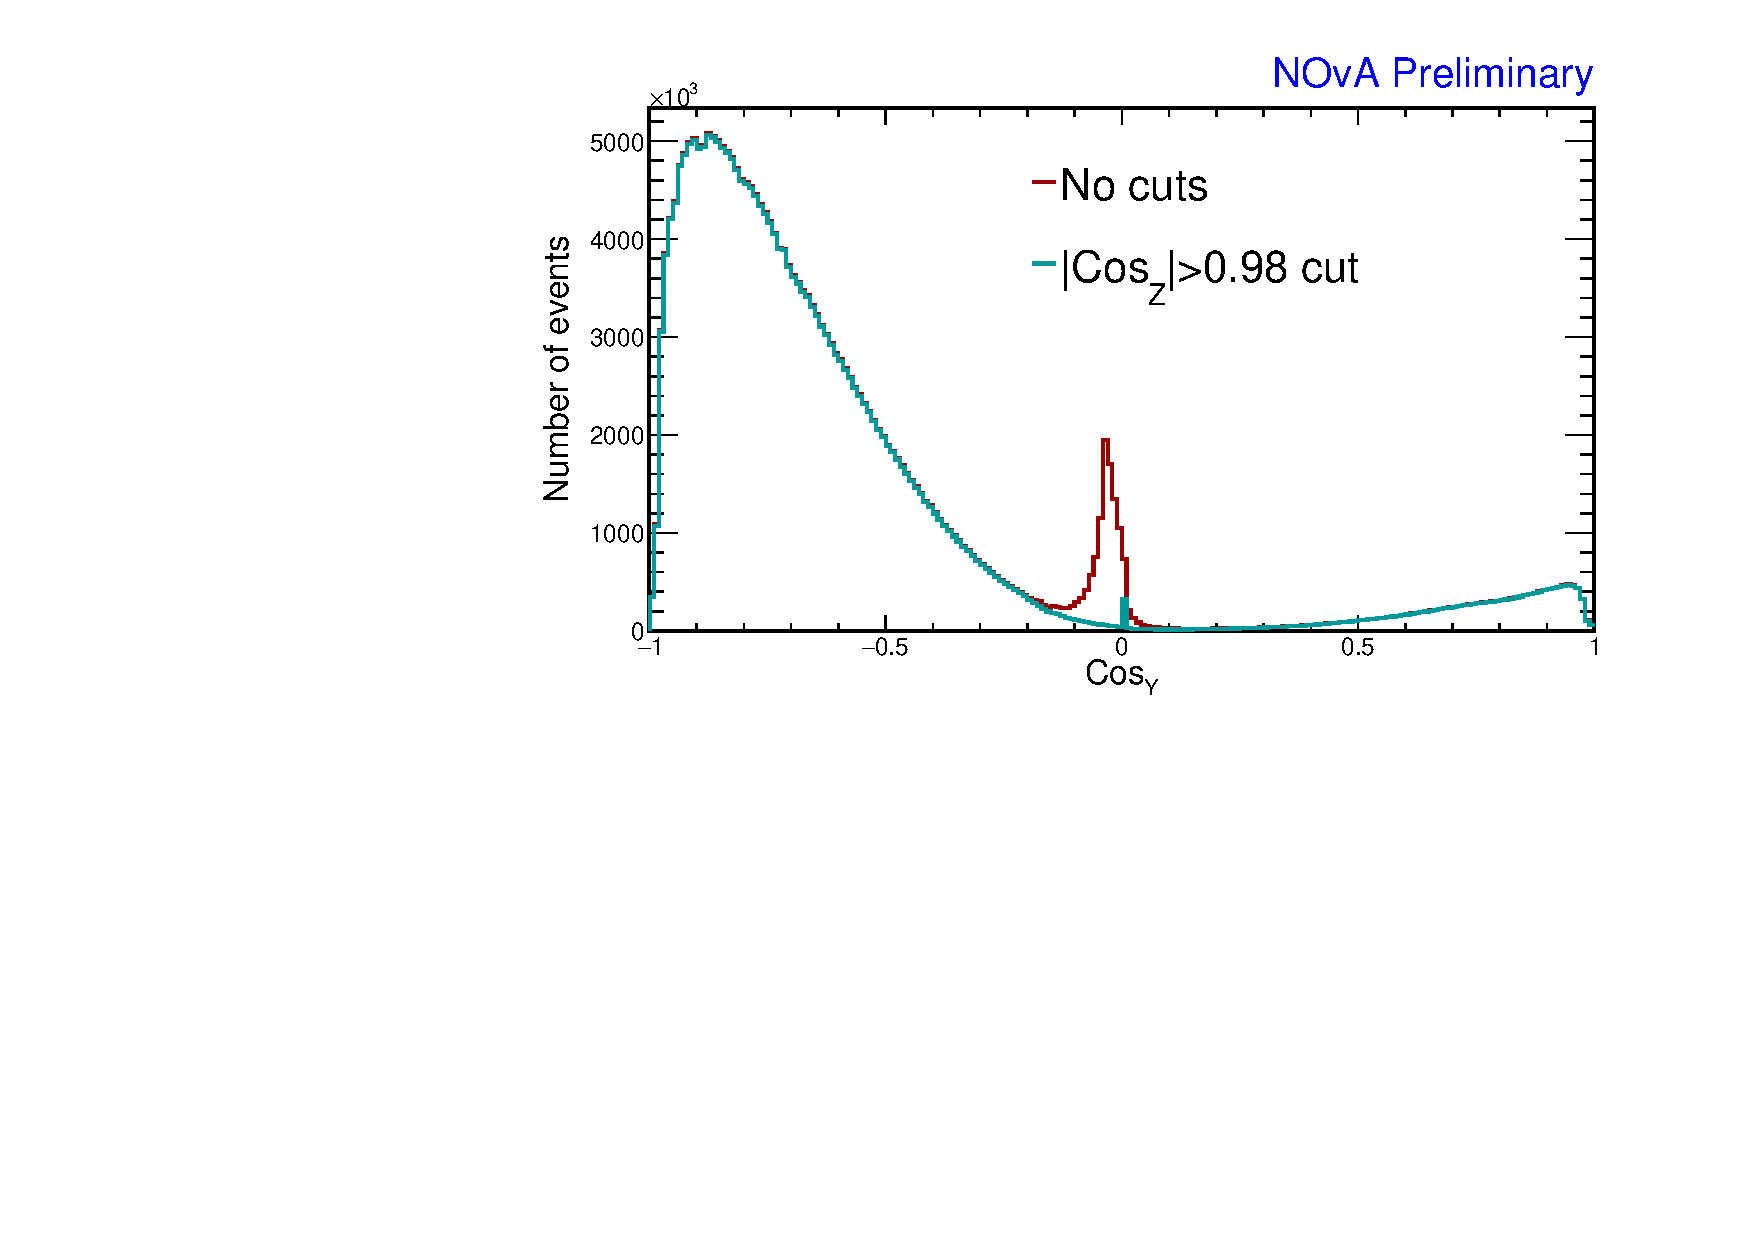
\includegraphics[width=\textwidth]{Plots/TBCalibration/DBSim_SelectionComparisonCosZCut_CosY.pdf}
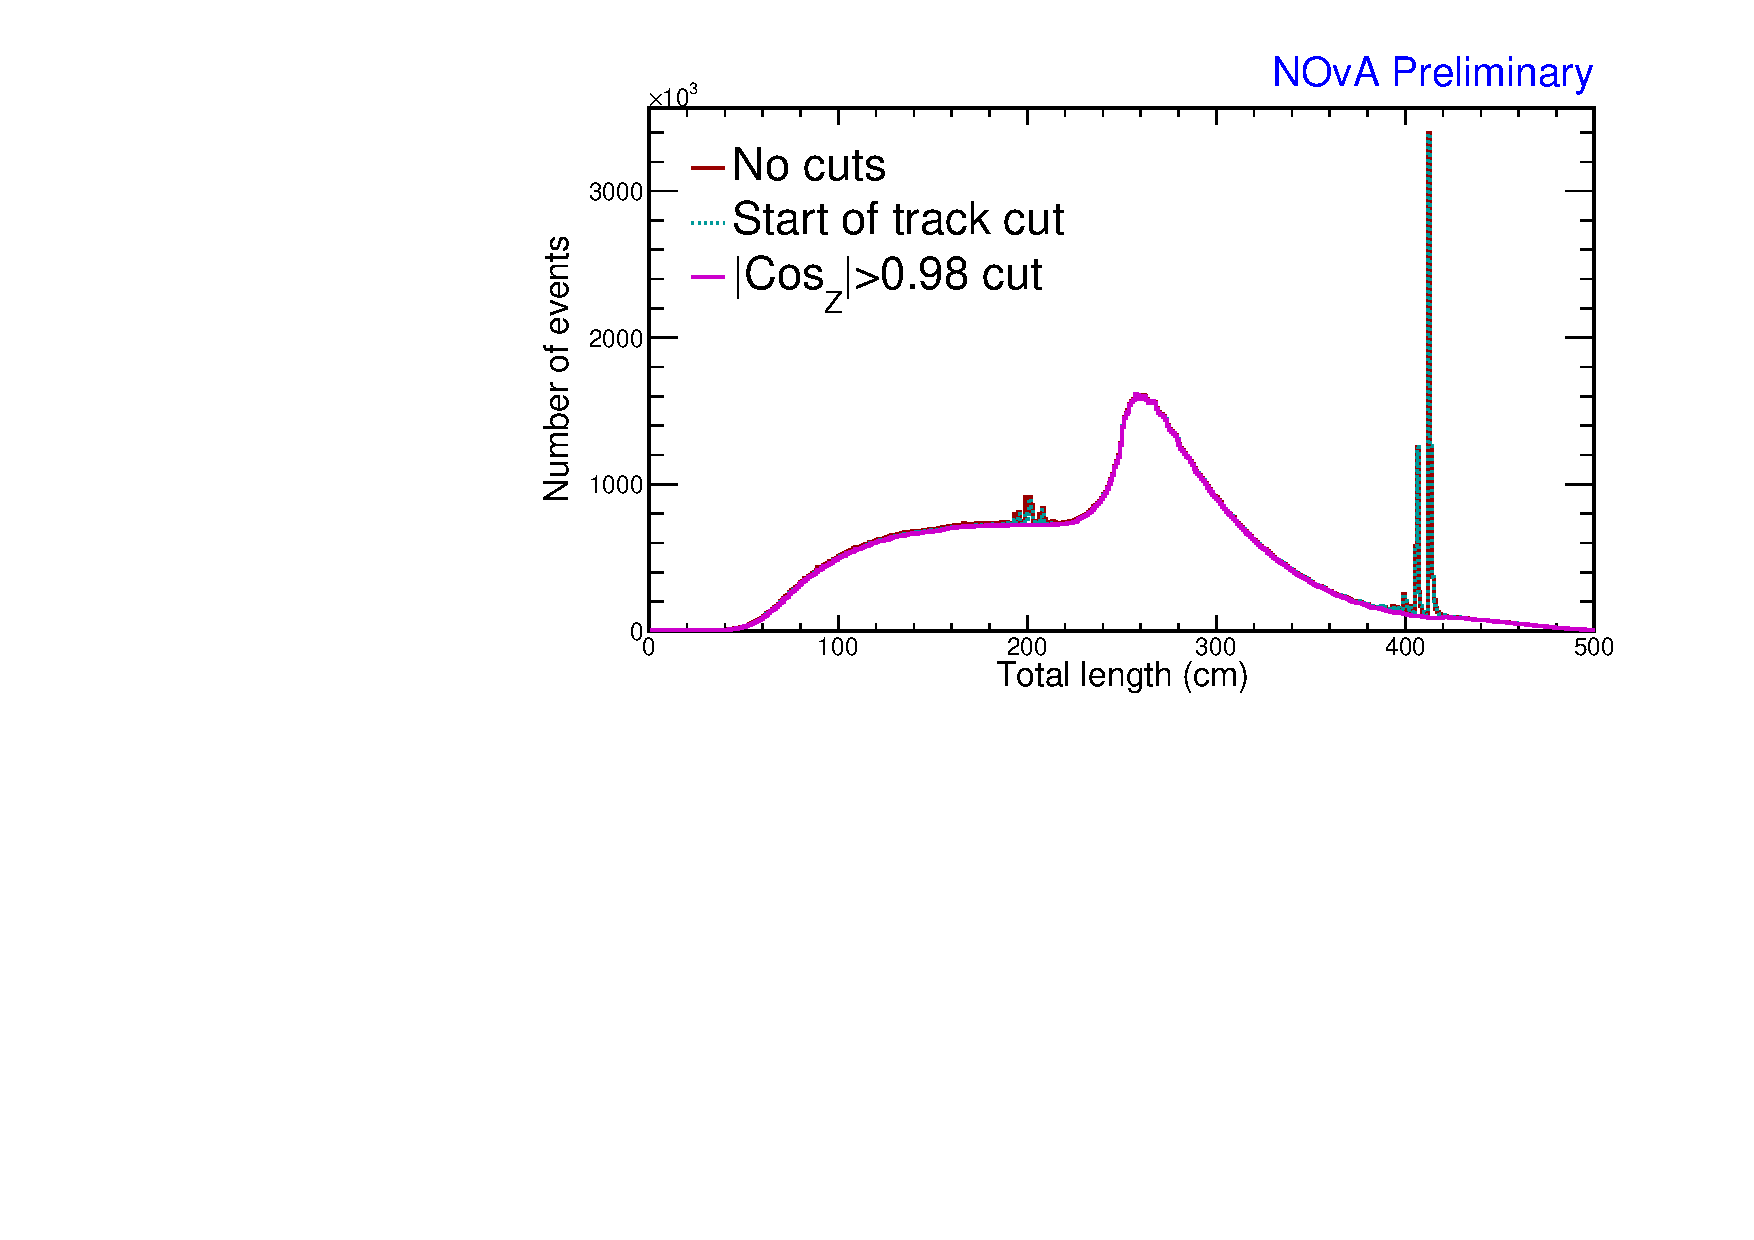
\includegraphics[width=\textwidth]{Plots/TBCalibration/DBSim_SelectionComparisonCosZCut_TotLength.pdf}
\caption[$\textsf{Cos}_Z$ cut for data-based simulation selection]{Impact of the cut on the maximum track angle from the z axis ($\textsf{Cos}_Z$) on the Test Beam data for the data-based simulation of cosmic muons. Top plot shows distribution of the angle from the y axis and bottom of the total track length, both made from the period 4 Test Beam data.}
\label{fig:DataBasedSimCosZSelectionComparison}
\end{figure}

\item We remove all events whose track is parallel to the beam direction, by requiring the angle from the z axis (parallel to the beam - labelled as $\textsf{Cos}_Z$ throughout text and plots for brevity) to be $|\textsf{Cos}_Z|\leq 0.98$. Figure \ref{fig:DataBasedSimCosZSelectionComparison} demonstrates the presence of events peaked at track lengths of approximately $\unit[410]{cm}$ and $\unit[200]{cm}$, which correspond to the total and half length of the detector, respectively (or alternatively lengths of both blocks and of a single block). These events are strictly parallel to the beam direction and are likely remnants of beam events. Applying a cut on $\textsf{Cos}_Z$ effectively removes these events without affecting the rest of the data. This cut might only be needed for the Test Beam detector and not for the \gls{ND} and \gls{FD}, as it is likely these are particles scattered from the Test Beam beamline, or from the secondary beam.

\item To ensure that only events contributing to the final calibration sample are simulated, we use a selection based on the cuts used to select events for the data calibration samples (described in Sec.~\ref{sec:NOvACalibration} and listed as Calibration sample selection in Tab.~\ref{tab:DataBasedSimEventSelection}). We call these cuts the \textbf{calibration cuts}. However, there are two caveats we need to consider when applying the calibration cuts:
\begin{enumerate}
\item First, to create calibration samples, we apply the selection on tracks from the \textbf{window cosmic track} algorithm instead of the \gls{BPF} algorithm, which yield different distributions as depicted in Fig.~\ref{fig:DataBasedSimTrackComparison}. Notably, the \gls{BPF} tracks have a hard cut-off at the detector edges, whereas the window cosmic tracks are allowed to start beyond these limits. Also, as can be seen in the bottom plot of Fig.~\ref{fig:DataBasedSimBPFPeaks}, the \gls{BPF} tracks have a ridged distribution in $\textsf{Cos}_Z$, which is not present for window cosmic tracks. The origin of this shape is not exactly known, but it is likely caused by the detector structure, as shown in Fig.~\ref{fig:DataBasedSimBPFPeaks}. We concluded that the ridged shape should not have any impact on the resulting simulation. However given these differences between the tracking algorithms, applying the calibration cuts on the \gls{BPF} tracks could mistakenly remove events that would pass the same selection when applied to the window cosmic tracks.

\begin{figure}[!ht]
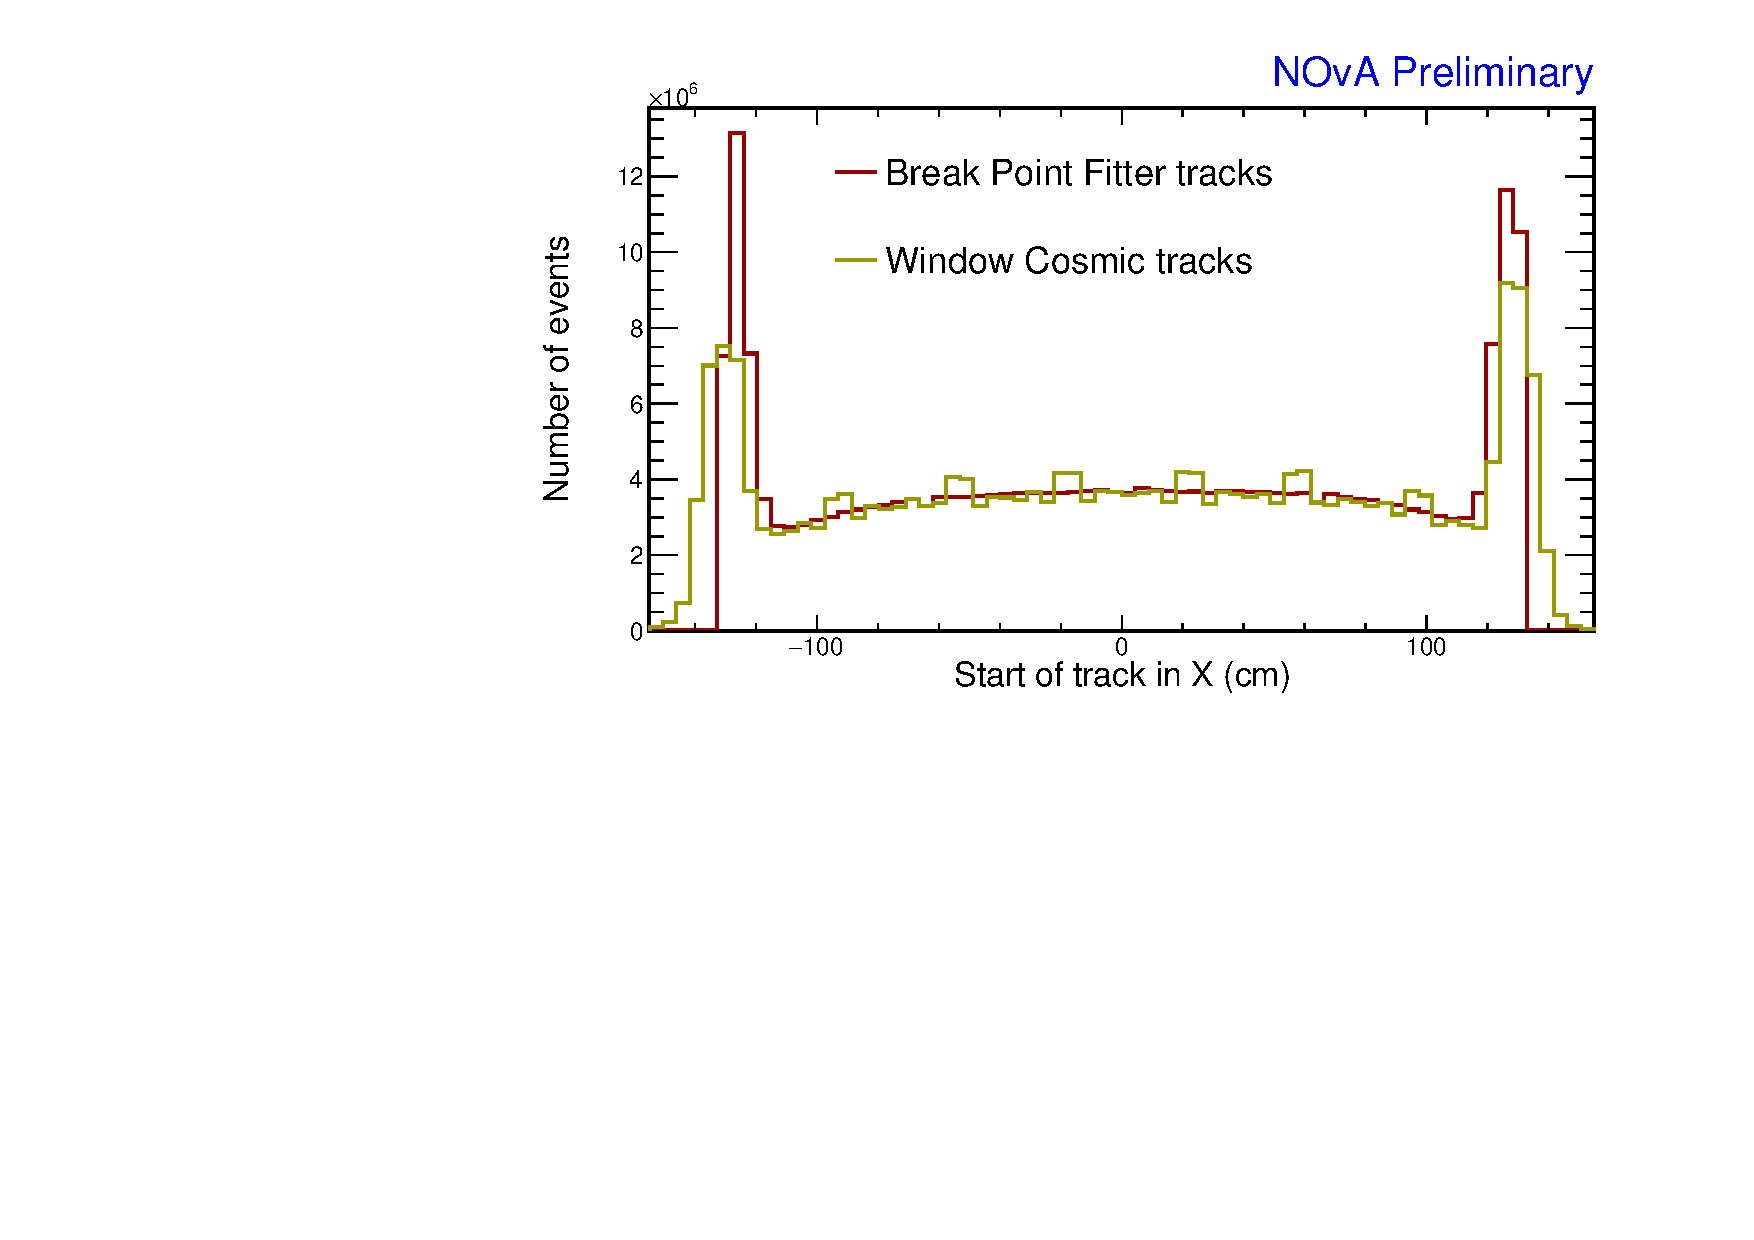
\includegraphics[width=\textwidth]{Plots/TBCalibration/DBSim_TrackAlgComparison_StartX.pdf}
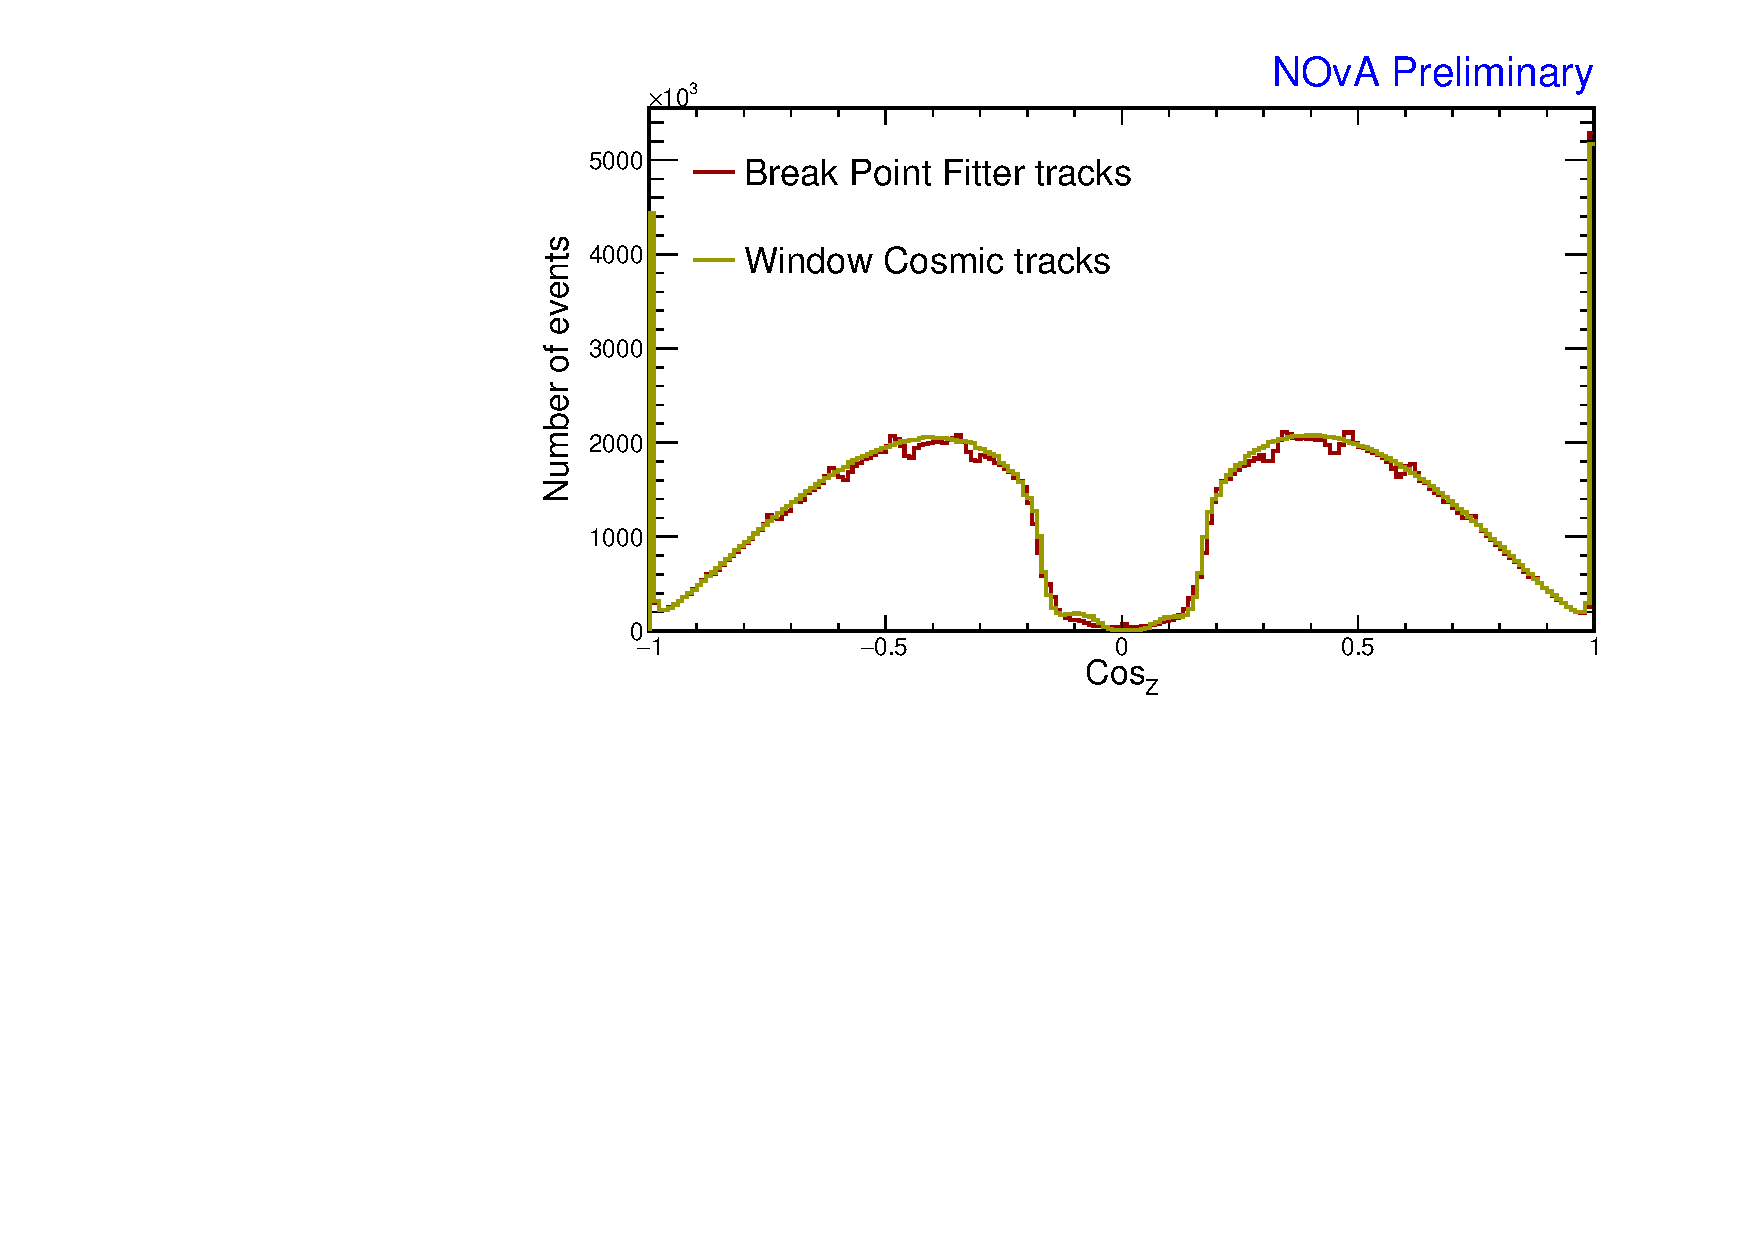
\includegraphics[width=\textwidth]{Plots/TBCalibration/DBSim_TrackAlgComparison_CosZ.pdf}
\caption[Tracking algorithms for the data-based simulation selection]{Difference between the tracks reconstructed with the \acrshort{BPF} and with the window cosmic track algorithms. Top plot shows the distribution of the start of track along the x axis and bottom plot shows the distribution of the angle from the z axis, both for the period 4 Test Beam data (with removed beam spill) without applying any selection.}
\label{fig:DataBasedSimTrackComparison}
\end{figure}

\begin{figure}[!hbtp]
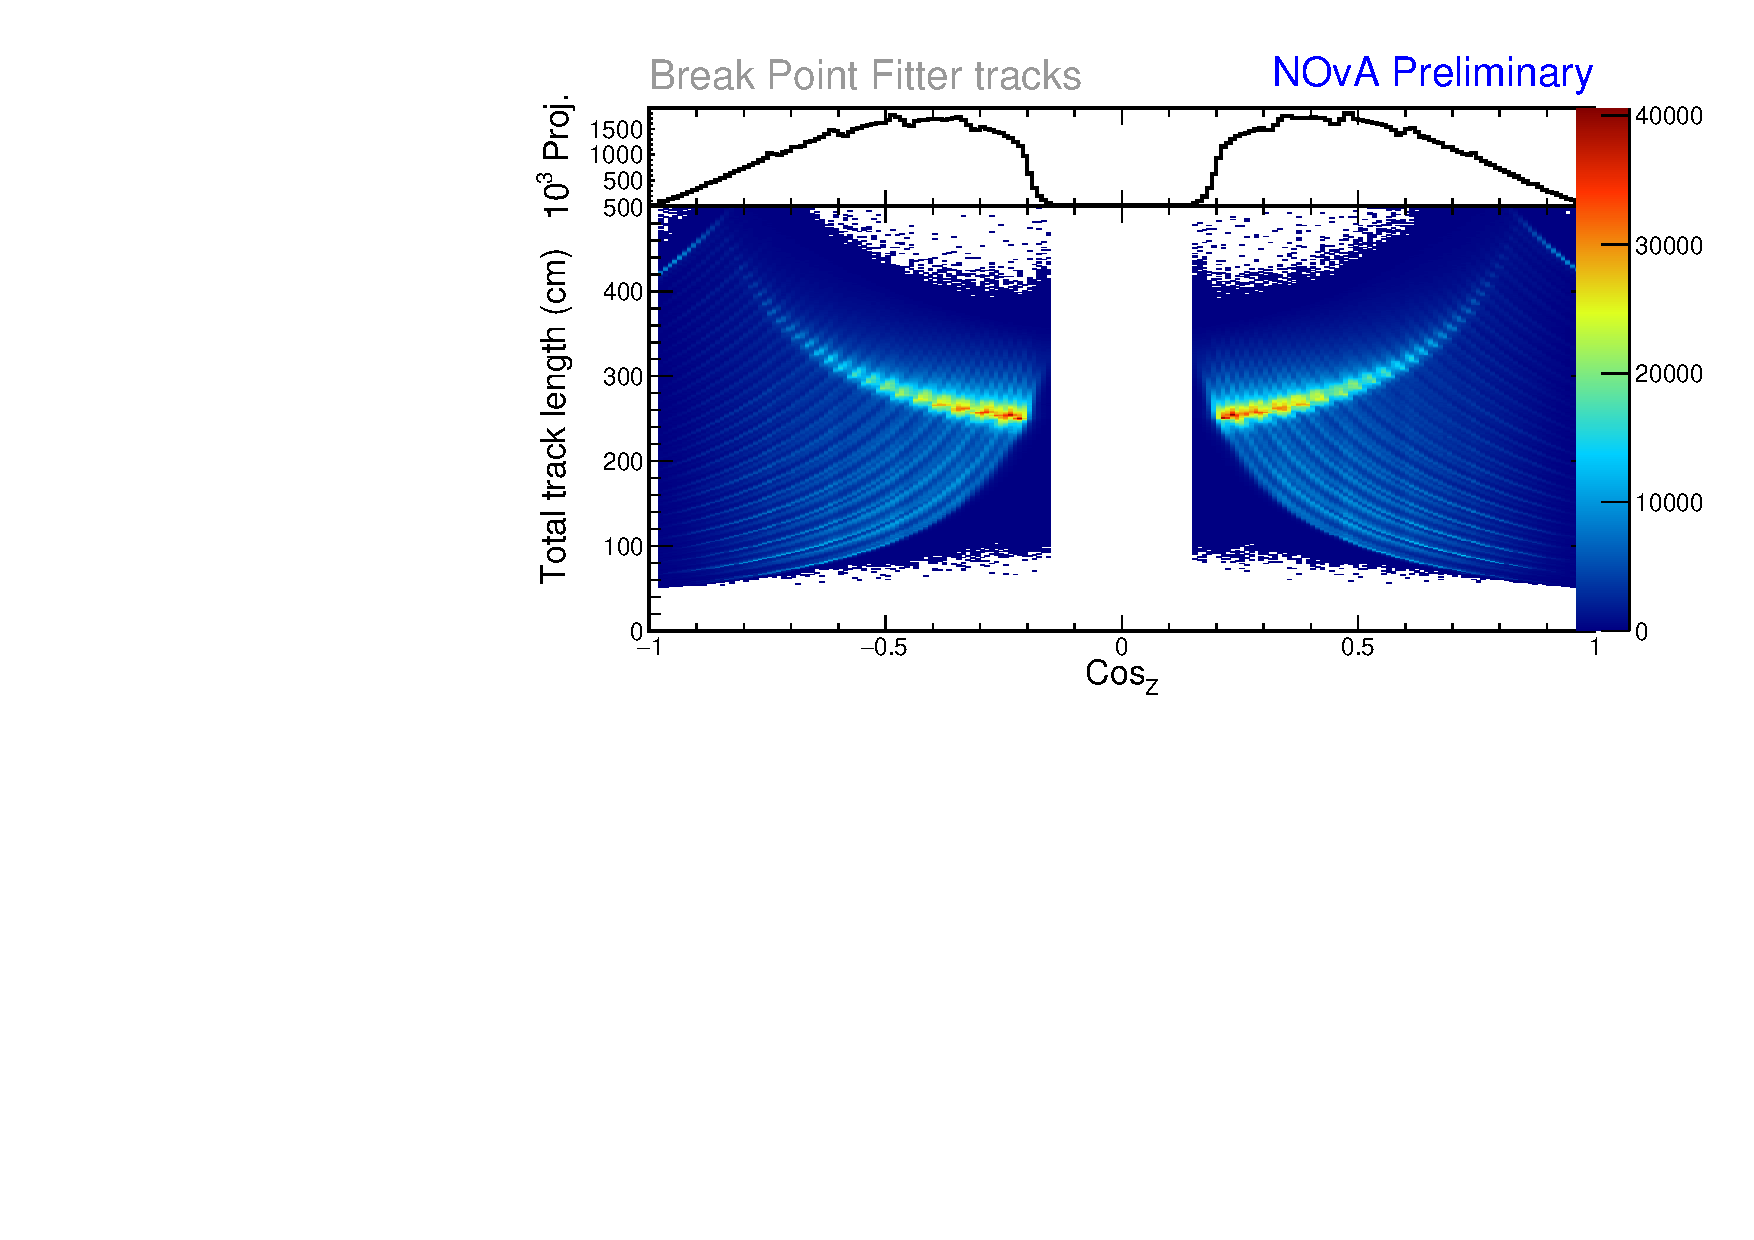
\includegraphics[width=\textwidth]{Plots/TBCalibration/DBSim_BPFPeaks_BPFTracks_dcosz_TotLength.pdf}
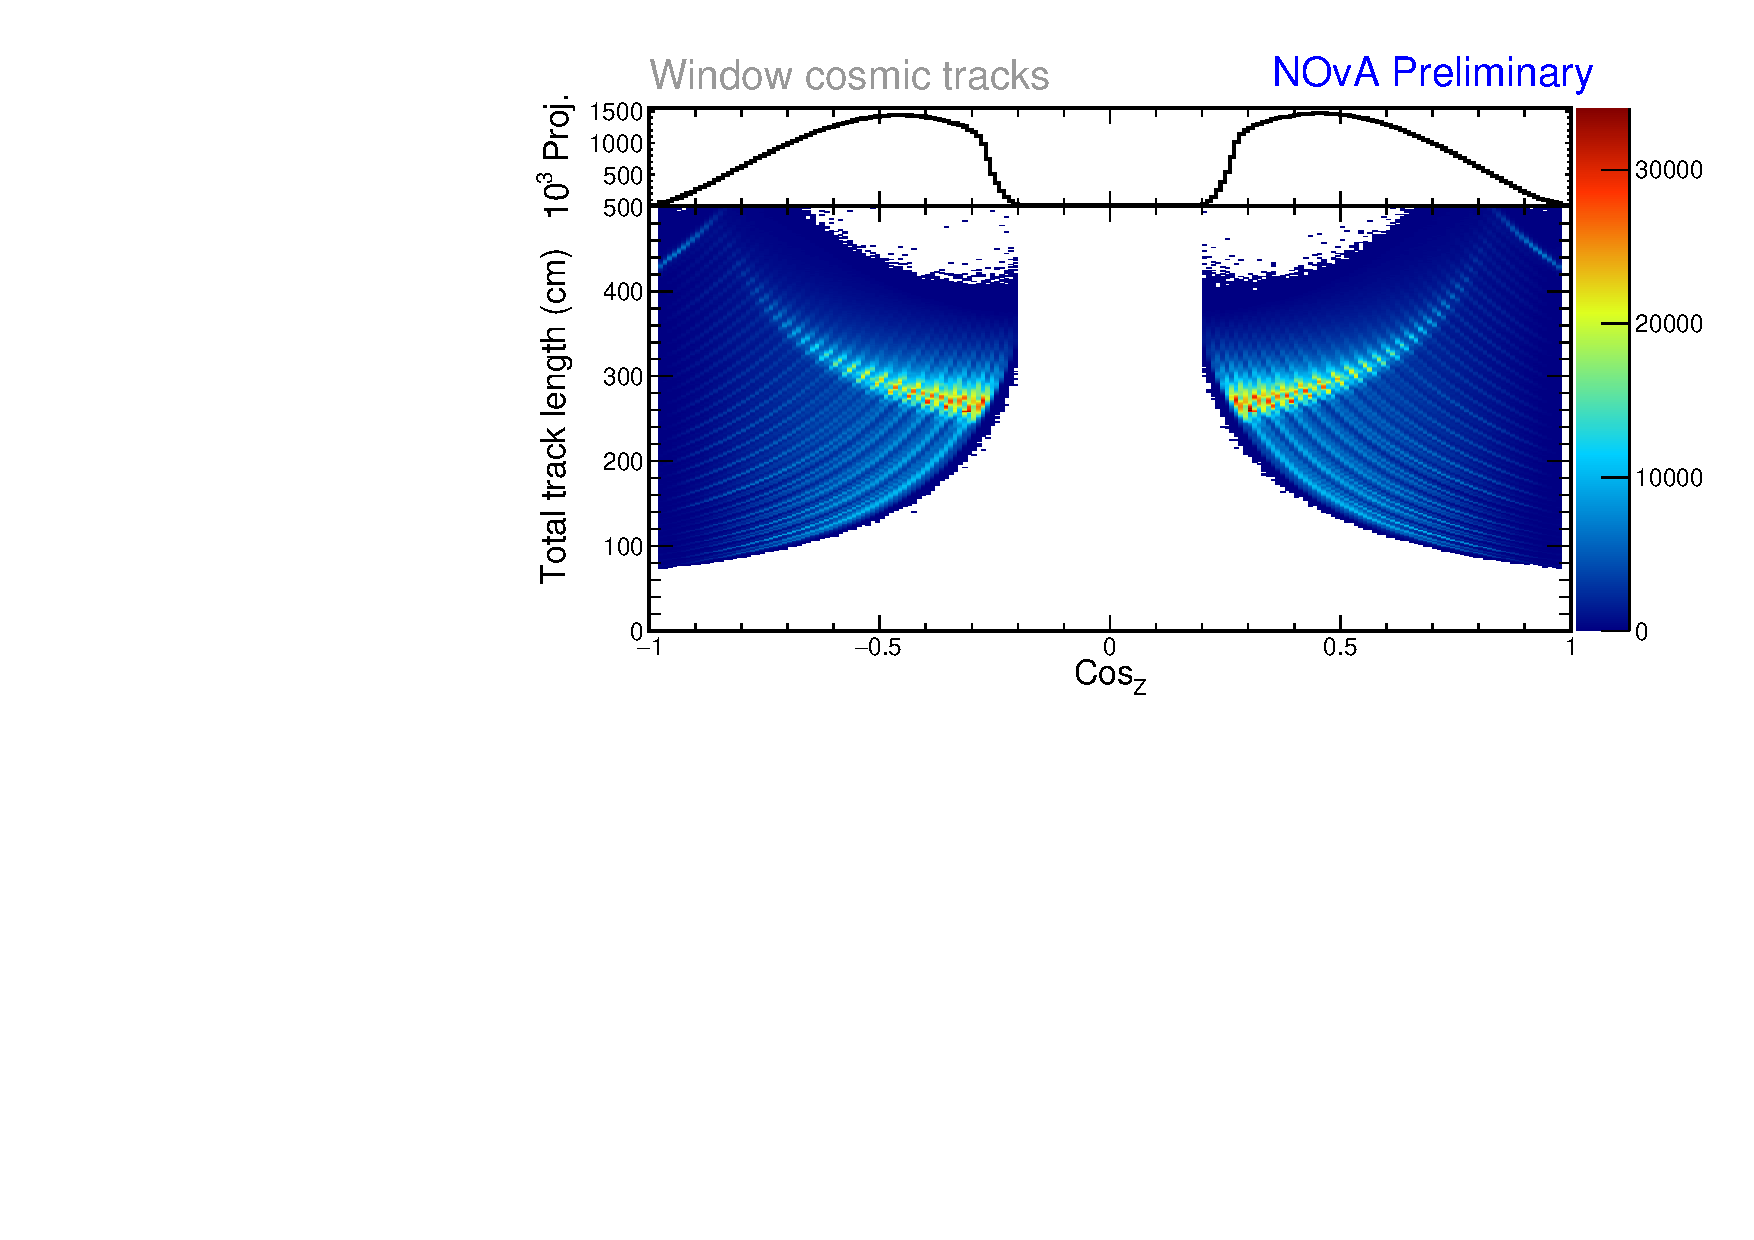
\includegraphics[width=\textwidth]{Plots/TBCalibration/DBSim_BPFPeaks_WTTracks_dcosz_TotLength.pdf}
\caption[Comparison of the $\textsf{Cos}_Z$ and track length distributions between tracking algorithms for the data-based simulation selection]{Comparison of the angle from the z axis ($\textsf{Cos}_Z$) and the total track length distributions between the \acrshort{BPF} tracks (top) and window cosmic tracks (bottom). Top parts of both plots show the 1D $\textsf{Cos}_Z$ distributions, scaled by $1/10^3$. The top plot is created with loose calibration cuts and the bottom plot with full calibration cuts per Tab.~\ref{tab:DataBasedSimEventSelection}, although this difference in selection shouldn't matter. These plots are investigating the origin of the ridged shape in the $\textsf{Cos}_Z$ distribution of \acrshort{BPF} tracks, as can be seen in the top part of the top plot. The long curved light blue/green lines in the 2D plots correspond to constant values of $\left|\textsf{Cos}_Z\right|\times\textsf{Tot. length} \equiv \textsf{Tot. length}_Z$, equal to the extent of the track length in the z direction, and are distinct from each other due to the structure of the detector (segmentation into planes). It is clear that the \gls{BPF} tracks are peaked more sharply in $\textsf{Tot. length}_Z$ than the window cosmic tracks, which are more spread out. This discrepancy could cause the resulting shape in the $\textsf{Cos}_Z$ distribution of \acrshort{BPF} tracks.}
\label{fig:DataBasedSimBPFPeaks}
\end{figure}

\item Second, each reconstruction algorithm has intrinsic deficiencies that can lead to misreconstructions. Therefore, applying the full calibration cuts on misreconstructed events may remove them, even though they would have passed if they were reconstructed correctly and hence they should have been included in the simulation. These events would then be missing from the resulting simulation sample, introducing a bias.
\end{enumerate}

To address these concerns, we loosened the full calibration cuts to create a `buffer' around the selected events, allowing for fluctuations of the reconstruction algorithms while maintaining track quality. This way, events that would have been removed based on the calibration cuts applied to their reconstructed \gls{BPF} tracks, but kept based on the calibration cuts applied to their window cosmic tracks, now have a chance to make it into the final selection and therefore calibration sample. The differences between the full calibration cuts and the employed loosened calibration cuts applied to the \gls{BPF} tracks are listed in Tab.~\ref{tab:DataBasedSimEventSelection} and shown in Fig.~\ref{fig:DataBasedSimCalibCutsComparison}. There we also show the data calibration sample, which was created by applying the full calibration cuts on window cosmic tracks.
\end{enumerate}

\iffalse
The cuts are:
\begin{itemize}
\item Tracks must have at least two X and two Y cells
\item The difference between the start and stop Z position of the track must be at least 70~cm
\item The Z component of the initial direction vector of the track must be at least 0.2
\item At least 80\% of cells in slice must be reconstructed into the track in both X and Y views
\item At most 6 cells were hit per plane
\item Maximum difference between the first planes in X and Y is 3 (same for the last planes)
\item The difference between number of planes crossed in X and Y view must be at most 10\% of the total number of planes crossed
\item Remove tracks where a step between trajectory points is more than this value * the median step size
\end{itemize}
\fi

\begin{table}[!ht]
\centering
\caption[Overview of the event selection for the data-based simulation]{Event selection of cosmic muons used for the data-based simulation (in green under Loose selection) and comparison to the Full selection cuts used to create the calibration samples (described in Sec.~\ref{sec:NOvACalibration}) in blue. The last two rows are not used for Test Beam, but are employed for the \acrshort{ND} and \acrshort{FD}.}
\begin{tabular}{clcc}
& \multirow{2}{*}{\centering{\textbf{Cut}}} & \multicolumn{2}{c}{\textbf{Selection}}\\
& & \cellcolor[HTML]{3166FF}\textbf{Full} & \cellcolor[HTML]{32CB00}\textbf{Loose}\\\hline
                                   & Muon assumption and 3D track from BPF         &                                             &                                          \\
                                   & Max. track start distance from edge                       & \multicolumn{2}{c}{50 cm}                                                                 \\
                                   & Max. $Cos_{Z}$                                            & \multicolumn{2}{c}{0.98}                                                               \\ \hline
                                   & Min. number of hits in X or Y                             & \multicolumn{2}{c}{\cellcolor[HTML]{FFFFFF}2}                                          \\
                                   & Min. difference between Stop$_{Z}$ and Start$_{Z}$        & \cellcolor[HTML]{3166FF}70~cm                 & \cellcolor[HTML]{32CB00}50~cm             \\
                                   & Min. $Cos_{Z}$ & \cellcolor[HTML]{3166FF}0.2                 & \cellcolor[HTML]{32CB00}0.15             \\
                                   & Min. frac. of slice hits in track in each view    & \multicolumn{2}{c}{0.8}                                                                \\
                                   & Max. number of cells per plane in each view               & \cellcolor[HTML]{3166FF}6                   & \cellcolor[HTML]{32CB00}15               \\
                                   & Max. difference in X-Y for first (last) plane     & \cellcolor[HTML]{3166FF}3                   & \cellcolor[HTML]{32CB00}5                \\
                                   & Max. plane asymmetry                                      & \cellcolor[HTML]{3166FF}0.1                 & \cellcolor[HTML]{32CB00}0.2              \\
                                   & Max. step size to median step size ratio                  & \cellcolor[HTML]{3166FF}3                   & \cellcolor[HTML]{32CB00}5                \\
                                   & \cellcolor[HTML]{C0C0C0}Max. vertex distance from edge    & \multicolumn{2}{c}{\cellcolor[HTML]{C0C0C0}10~cm}                                         \\
\parbox[t]{2mm}{\multirow{-10}{*}{\rotatebox[origin=c]{90}{Calibration sample selection}}}& \cellcolor[HTML]{C0C0C0}Max. track end distance from edge & \multicolumn{2}{c}{\cellcolor[HTML]{C0C0C0}10 cm}
\end{tabular}
\label{tab:DataBasedSimEventSelection}
\end{table}

\begin{figure}[!h]
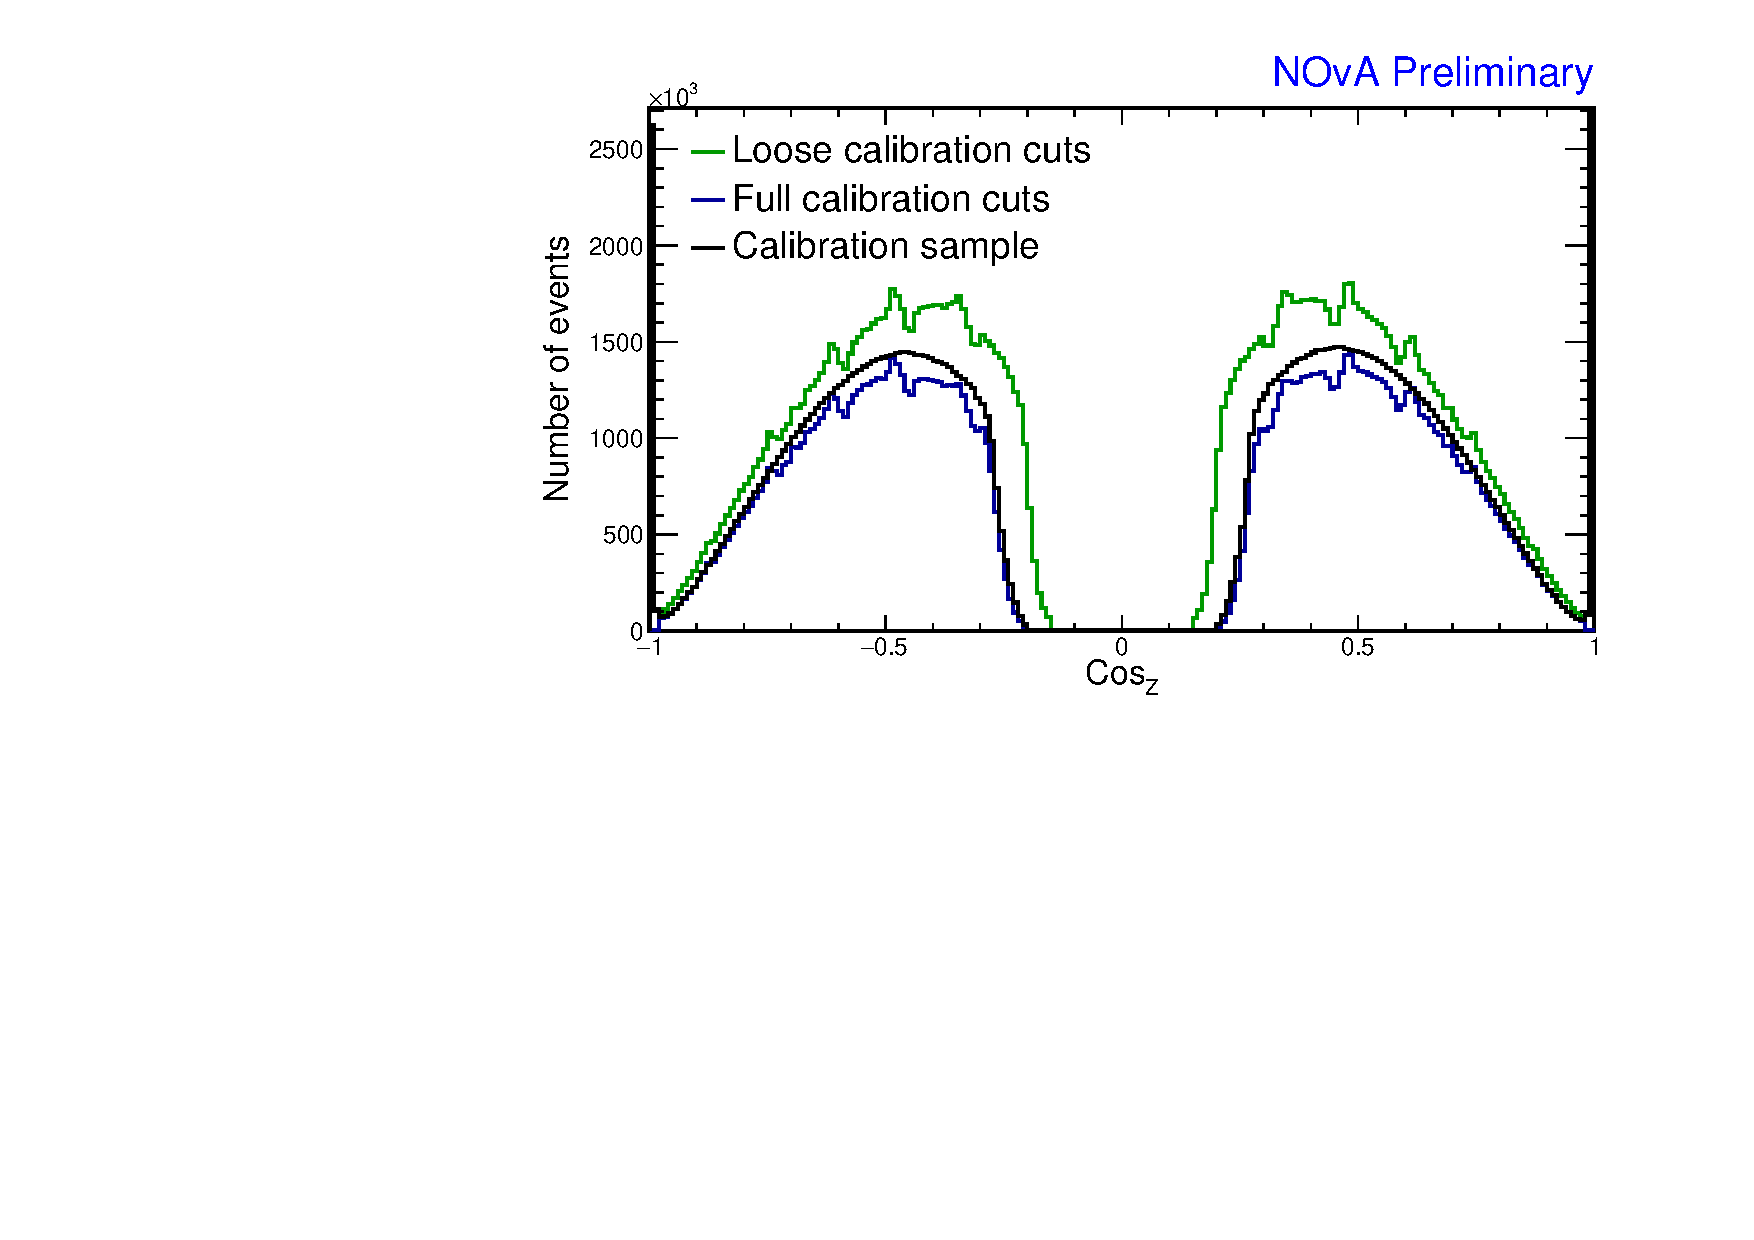
\includegraphics[clip, width=\textwidth]{Plots/TBCalibration/DBSim_SelectionComparisonPCHitsListCut_CosZ.pdf}
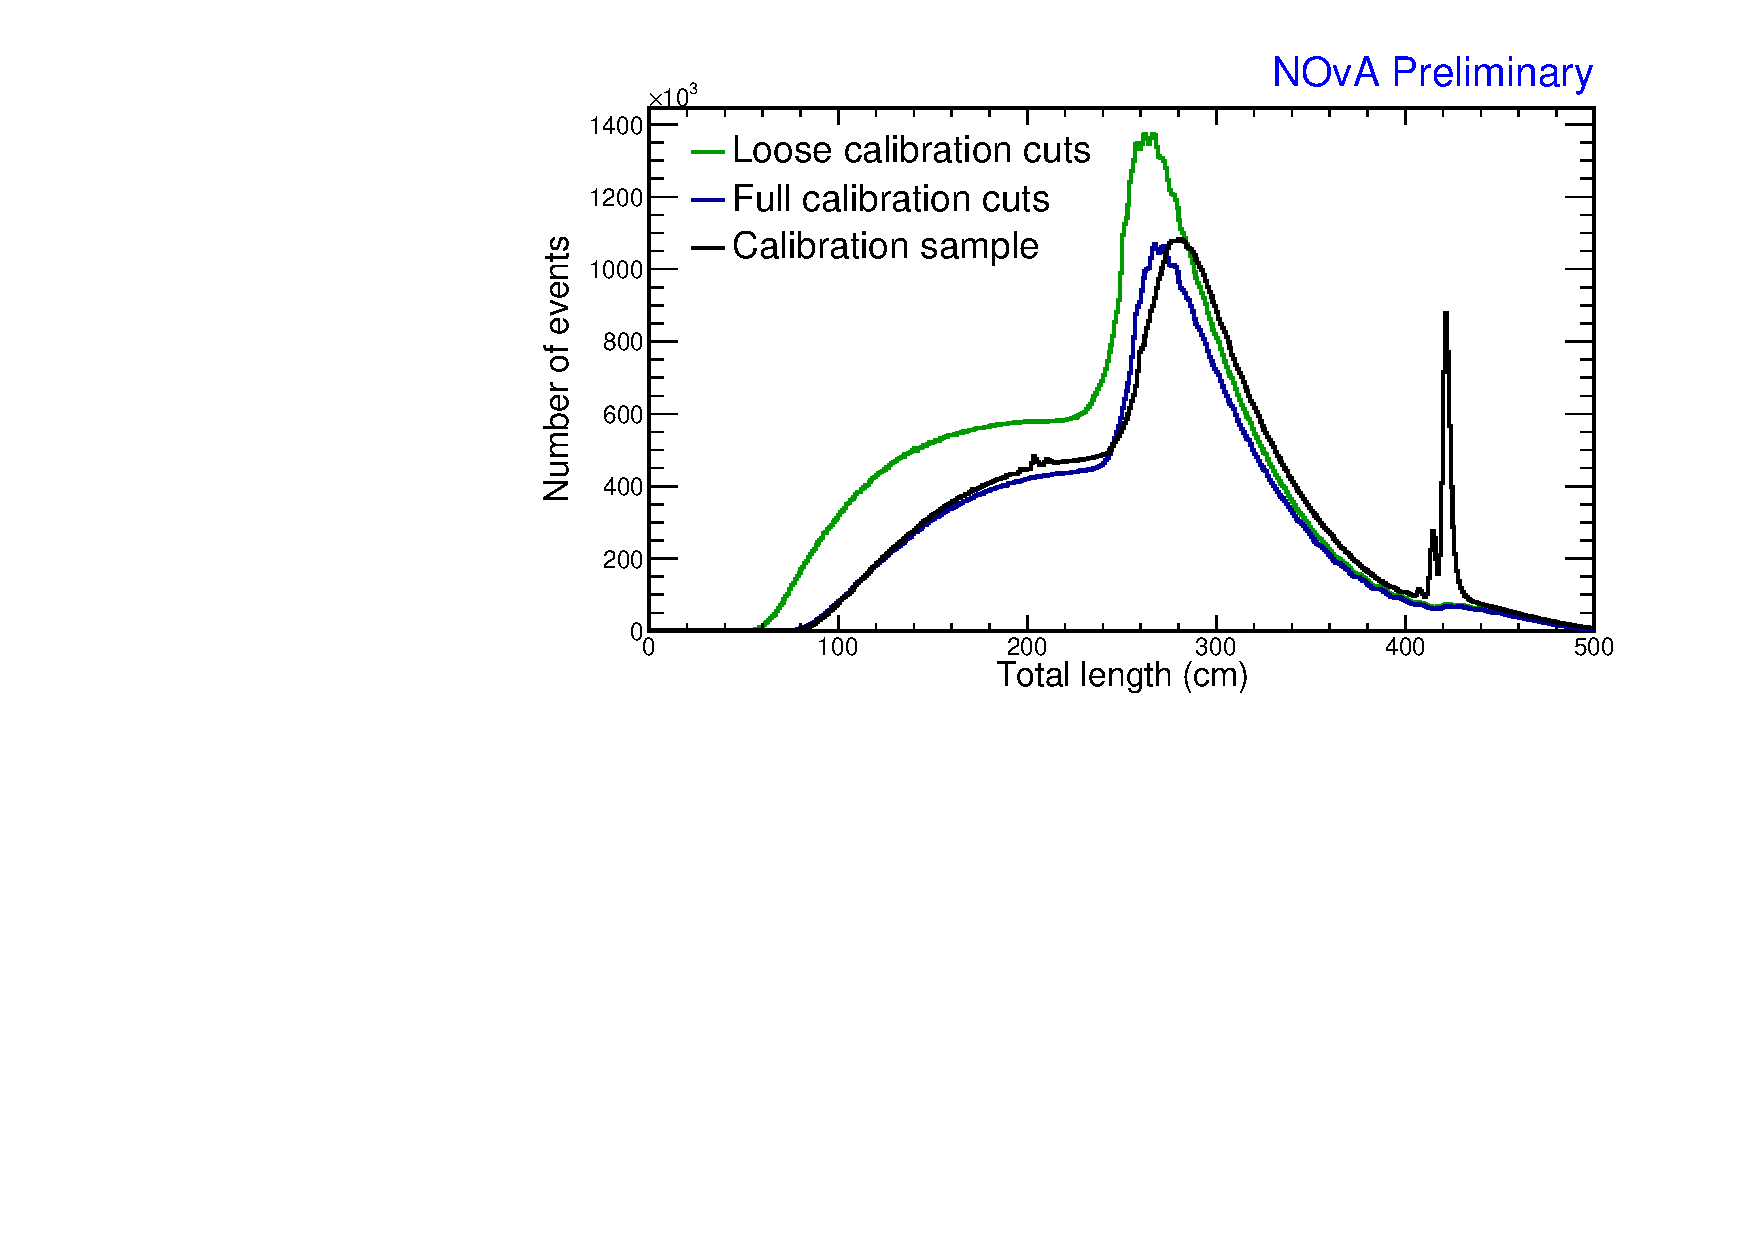
\includegraphics[clip, width=\textwidth]{Plots/TBCalibration/DBSim_SelectionComparisonPCHitsListCut_TotLength.pdf}
\caption[Event selection for the data-based simulation]{Comparison of full and loose event selections for the data-based simulation as per Tab.~\ref{tab:DataBasedSimEventSelection} and of the corresponding data calibration sample in black. As described in text, the loose calibration cuts applied to the \acrshort{BPF} tracks (green) were used for simulation to mitigate the discrepancy between applying the full calibration cuts to the \acrshort{BPF} tracks (blue) and the window cosmic tracks (black). All of the distributions are made from the period 4 Test Beam data.}
\label{fig:DataBasedSimCalibCutsComparison}
\end{figure}

During the selection process, we determine whether the muon is stopping inside the detector or passing through, based on the end position of the reconstructed track. For Test Beam we say it is a stopping muon if its track ends at least $\unit[20]{cm}$ from any edge of the detector. For the \gls{ND} and \gls{FD} this is $\unit[50]{cm}$. This information assists in correcting the energy of through-going muons, as outlined in the following Sec.~\ref{sec:DataBasedSimPython}.

%\FloatBarrier
\section{Energy correction, charge assignment and smearing}\label{sec:DataBasedSimPython}
Once we have the kinematic information for the selected events, we perform several tasks to get the final sample of cosmic muons for the data-based simulation. This includes correcting energies of the through-going muons, assigning a charge to each muon event, and smearing and converting the information into the correct format required by the generator.

\subsection*{Energy correction}
Through-going muons do not deposit all of their energy inside the detector. Therefore we cannot reliably calculate their initial energies from the reconstructed information, but we can estimate an energy that could leave the same track. In general, the energy spectrum of cosmic muons can be approximately described by a power law $E^{-\alpha}$, with $\alpha\approx2.7$ \cite{NOvA-doc-51327,PDG.pdf}. The expectation value for the `true' initial energy of through-going muons can be therefore calculated as
\begin{equation}
\left\langle E\right\rangle =\frac{\int^{E_C}_{E_R} E\cdot E^{-\alpha}}{\int^{E_C}_{E_R} E^{-\alpha}}=\left(\frac{\alpha -1}{\alpha -2}\right)\left(\frac{E_C^{2-\alpha}-E_R^{2-\alpha}}{E_C^{1-\alpha}-E_R^{1-\alpha}}\right),
\end{equation}
where $E_R$ is the reconstructed energy we got from the \gls{BPF}. $E_C$ is the critical energy chosen conservatively to be $\unit[300]{GeV}$, as we do not expect muons with higher energies to be selected due to large showers along their paths. We use this corrected initial energy for all muons that do not stop inside the detector, as identified during selection described in Sec.~\ref{sec:DataBasedSimSelection}. Figure \ref{fig:DataBasedSimEnergyScaling} shows the corrected energy distribution of our selected events and demonstrates that the choice of the critical energy does not significantly change the correction. 

\begin{figure}[hbtp]
\centering
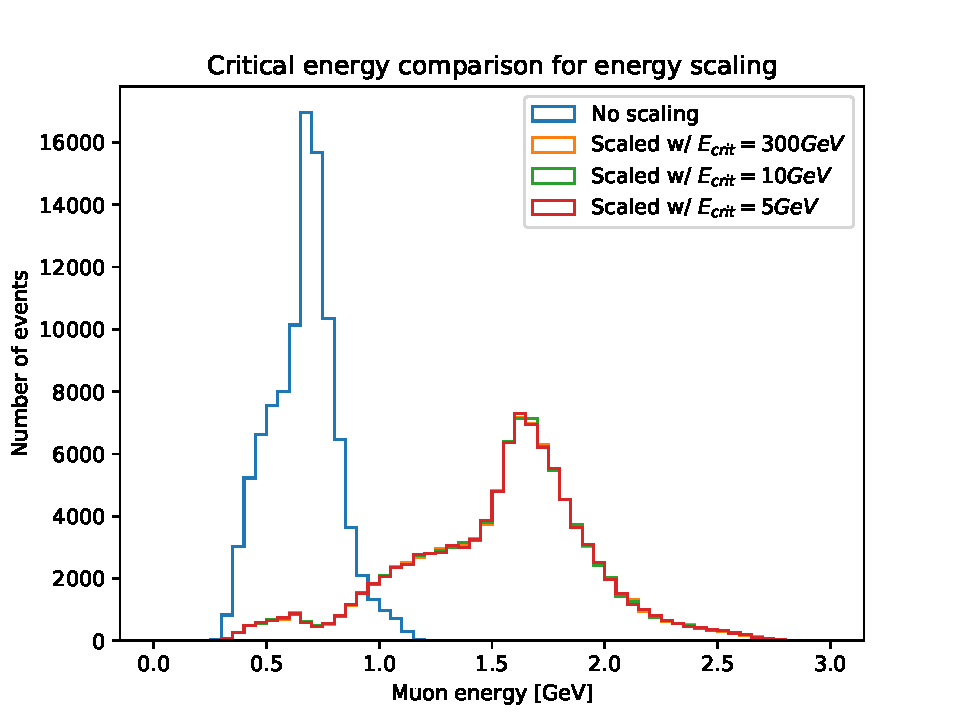
\includegraphics[width=0.8\textwidth]{Plots/TBCalibration/DBSim_ECritComparison.pdf}
\caption[Energy correction for through-going muons for the data-based simulation]{The effect of energy correction for through-going muons with various critical energies. No significant difference can be seen when using different critical energies.}
\label{fig:DataBasedSimEnergyScaling}
\end{figure}

This corrected energy is however \textbf{not} a good representation of the true energy spectrum of cosmic muons at surface level and getting a correct energy distribution from data would require a much more dedicated effort. The corrected energy would also be different for different \gls{NOvA} detectors, since the reconstructed energy is calculated from the track length. For example, the corrected energy of cosmic muons when entering the detector would be larger for the bigger \gls{ND} than for Test Beam, even though the \gls{ND} is underground. 

However, since this simulation is intended to be used for calibration, where we use through-going muons only for relative calibration, we do not need a perfect representation of the cosmic muon energy spectrum. Not including more energetic cosmic muons into the simulation does bias the energy deposition towards lower values, but this is corrected for during absolute calibration which only uses stopping muons, for which we assume we reconstruct their energy well from \gls{BPF}.

If someone were to use this simulation for something other than calibration, it would be necessary to rethink the energy correction, either by changing the energy estimation from track based algorithms to energy deposition, or by including information from external sources. It would also be necessary to include angular dependence for the energy correction as described in the PDG \cite{PDG.pdf}.

\subsection*{Smearing}
The reconstructed distributions in data are influenced by the detector structure, reconstruction efficiencies and other effects that can bias the simulation. To avoid this influence, we smear the reconstructed values by randomly varying
\begin{itemize}
\item the total momentum within 2\%,
\item the azimuthal angle uniformly,
\item the polar angle within $\unit[4]{mrad}$,
\item and the x, y and z vertex positions within the width or depth of the cell respectively.
\end{itemize}

\subsection*{Charge assignment}
We need to tell the detector simulation whether to simulate a muon or an anti-muon. However we do not reconstruct the charge of the muons, so we have to randomly assign it based on a statistical distribution from external measurements. The probability that a muon has a positive charge can be expressed as \cite{NOvA-doc-51327} 

%Figure out where are the plots and the equation Mark/Teresa quoted from (somewhere in PDG). Describe the basis of the measurement.
%Here(p10): https://pdg.lbl.gov/2022/reviews/rpp2022-rev-cosmic-rays.pdf
%But the equation must be from one of the sources listed.

\begin{equation}
P_+ \simeq 0.539 + \frac{x}{34.5}-\left(\frac{x}{9.48}\right)^2 + \left(\frac{x}{8.27}\right)^3,
\end{equation}
where $x$ is the logarithm of the total momentum in $\unit{GeV}$.

\subsection*{Production of the simulation}
We save the vertex positions, the four momenta and the assigned charge into a text file, that is then fed into the same detector and readout simulation chain, as was described for the \gls{ND} and \gls{FD} in Sec.~\ref{sec:NOvASimulation}.  We use the fibre brightness map that is used in calibration (see Sec.~\ref{sec:NOvACalibration}) to inform the simulation about the real detector conditions. Since we want the simulated detectors to be functional copies of the ideal versions of the real detectors, it is important to provide a correct brightness file without any defects. For this simulation we use the fibre brightness map described in Sec.~\ref{sec:FibreBrightnessTB}.

\section{Validation}\label{sec:DataBasedSimValidation}
To validate whether the newly created simulation works as expected, we create the simulation calibration sample using the reconstruction and selection of cosmic muons for calibrations described in Sec.~\ref{sec:NOvACalibration}. We then compare this to the equivalent data calibration sample, created from the same data that was used to seed the simulation. Additionally, we use the newly simulated events as `fake data' and pass them through the same reconstruction, selection and simulation processes as were used to create the first iteration, hence creating a `re-simulation' sample. This is used to validate the stability of the simulation process.

The data-simulation comparisons are shown in Fig.~\ref{fig:DataBasedSimDataMCComparison_cosXcosY}-\ref{fig:DataBasedSimDataMCComparison_startZ}. The data and simulation calibration samples are shown in black and pink solid lines respectively. Both are equivalent to applying the full calibration cuts to the window cosmic tracks, as described in Sec.~\ref{sec:DataBasedSimSelection}. For comparison, we are also showing distributions of the \gls{BPF} tracks with full and loose calibration cuts in blue and green dashed lines respectively. We are expecting that the distributions of the simulation calibration sample (pink) match the distributions of the data calibration sample (black), without being affected by the different shape of the \gls{BPF} tracks (dashed lines).

\begin{figure}[!ht]
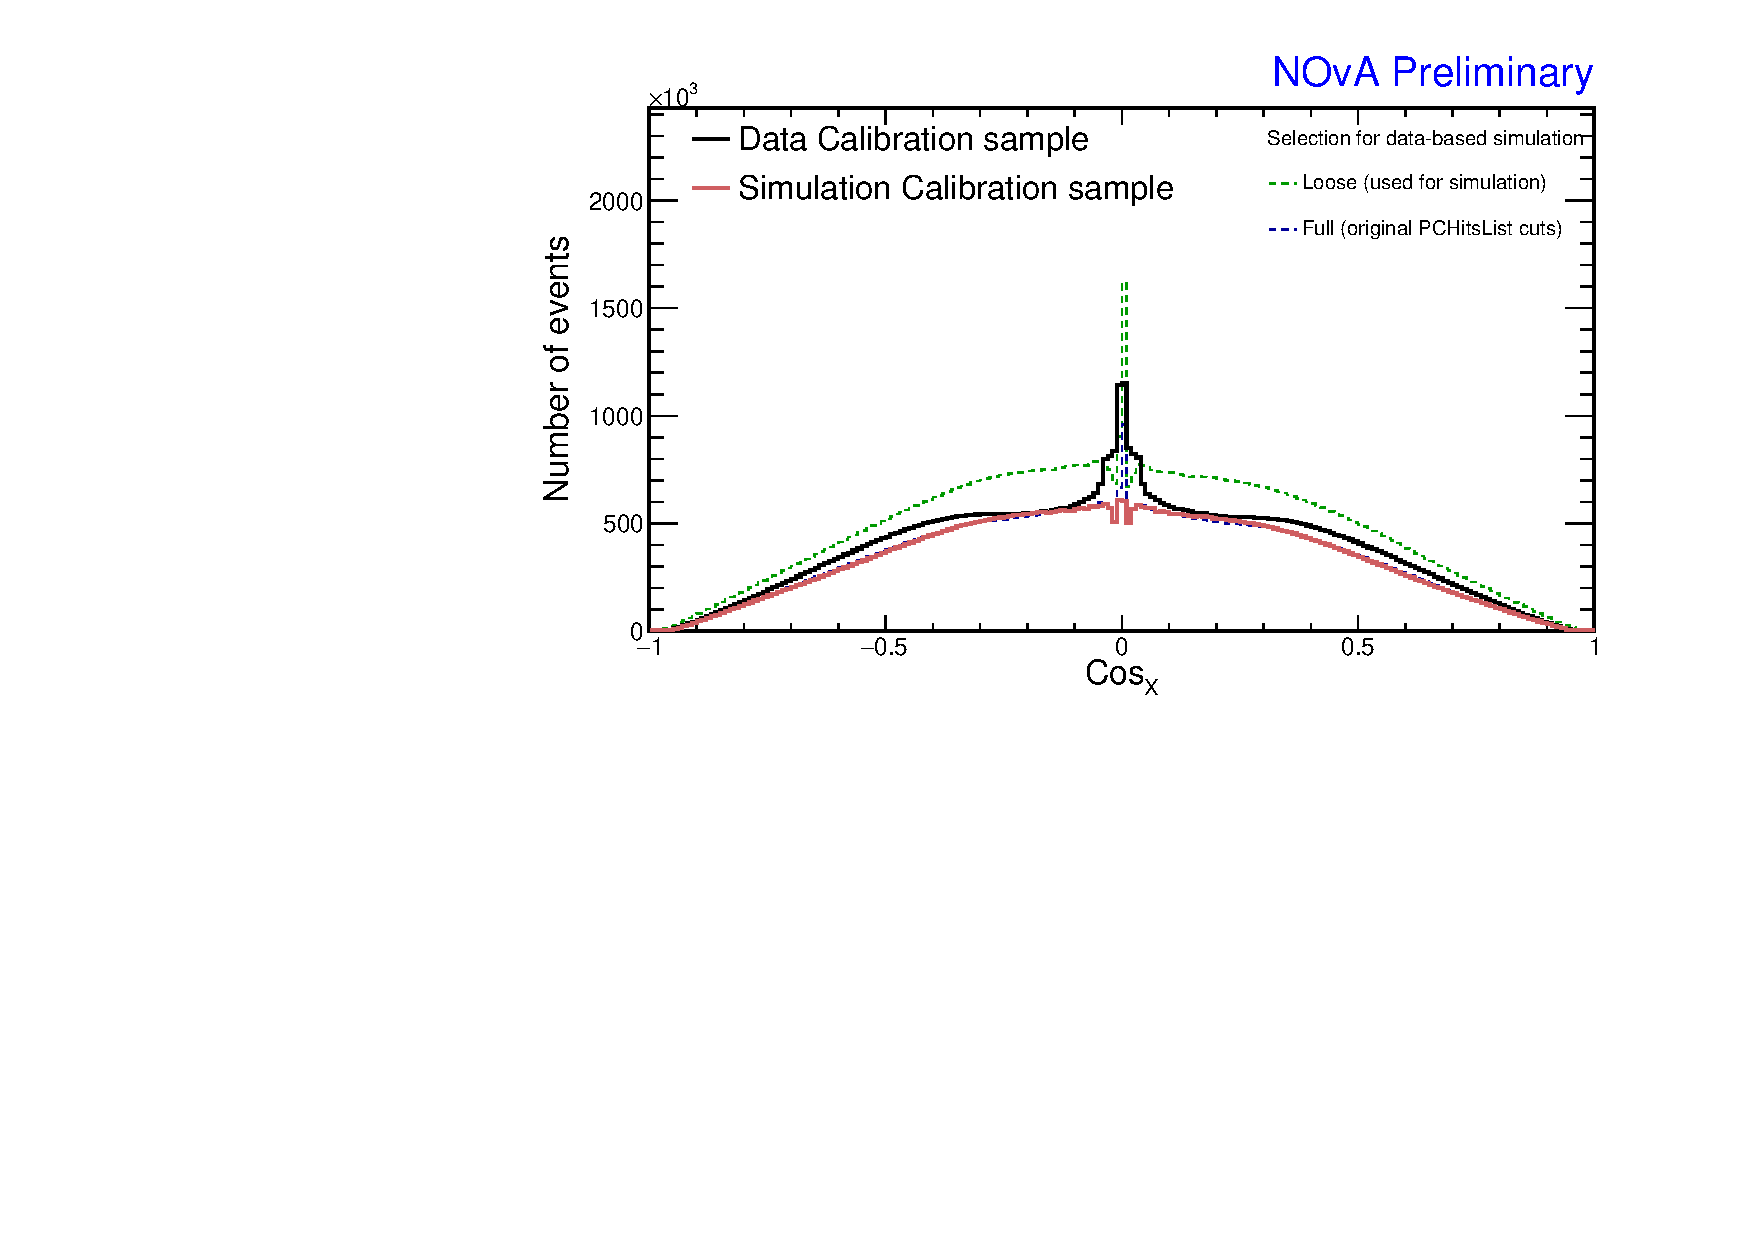
\includegraphics[width=\textwidth]{Plots/TBCalibration/DBSim_DataMCComparison_CosX.pdf}
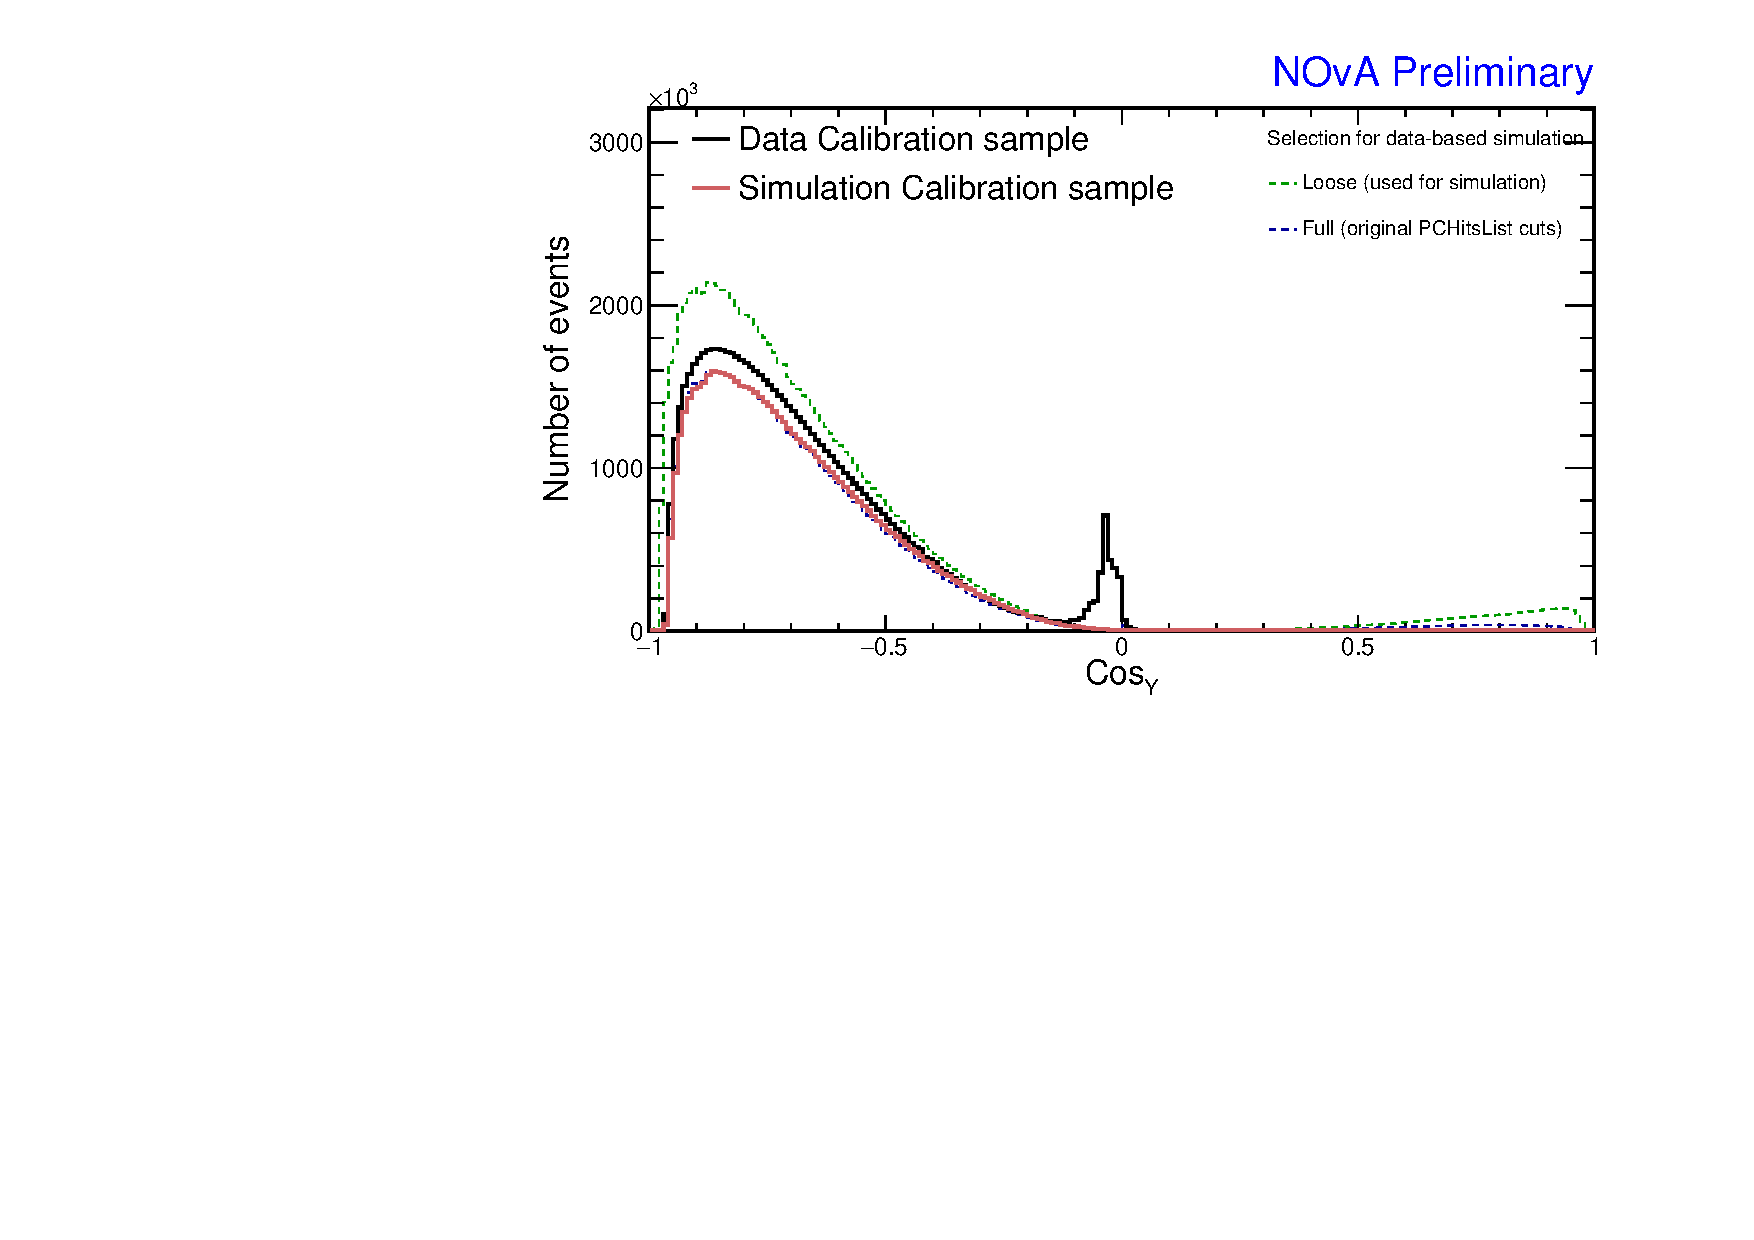
\includegraphics[width=\textwidth]{Plots/TBCalibration/DBSim_DataMCComparison_CosY.pdf}
\caption[Data-Simulation comparison of angular distributions]{Comparison of the angle from the x axis (top) and y axis (bottom) between the data (black) and simulation (pink) calibration samples, as detailed in the text. Additionally, the distributions of data with full (blue) and loose (green) selections applied to the \acrshort{BPF} tracks are shown, where the loose selection was used to create the simulation.}
\label{fig:DataBasedSimDataMCComparison_cosXcosY}
\end{figure}

\begin{figure}[!ht]
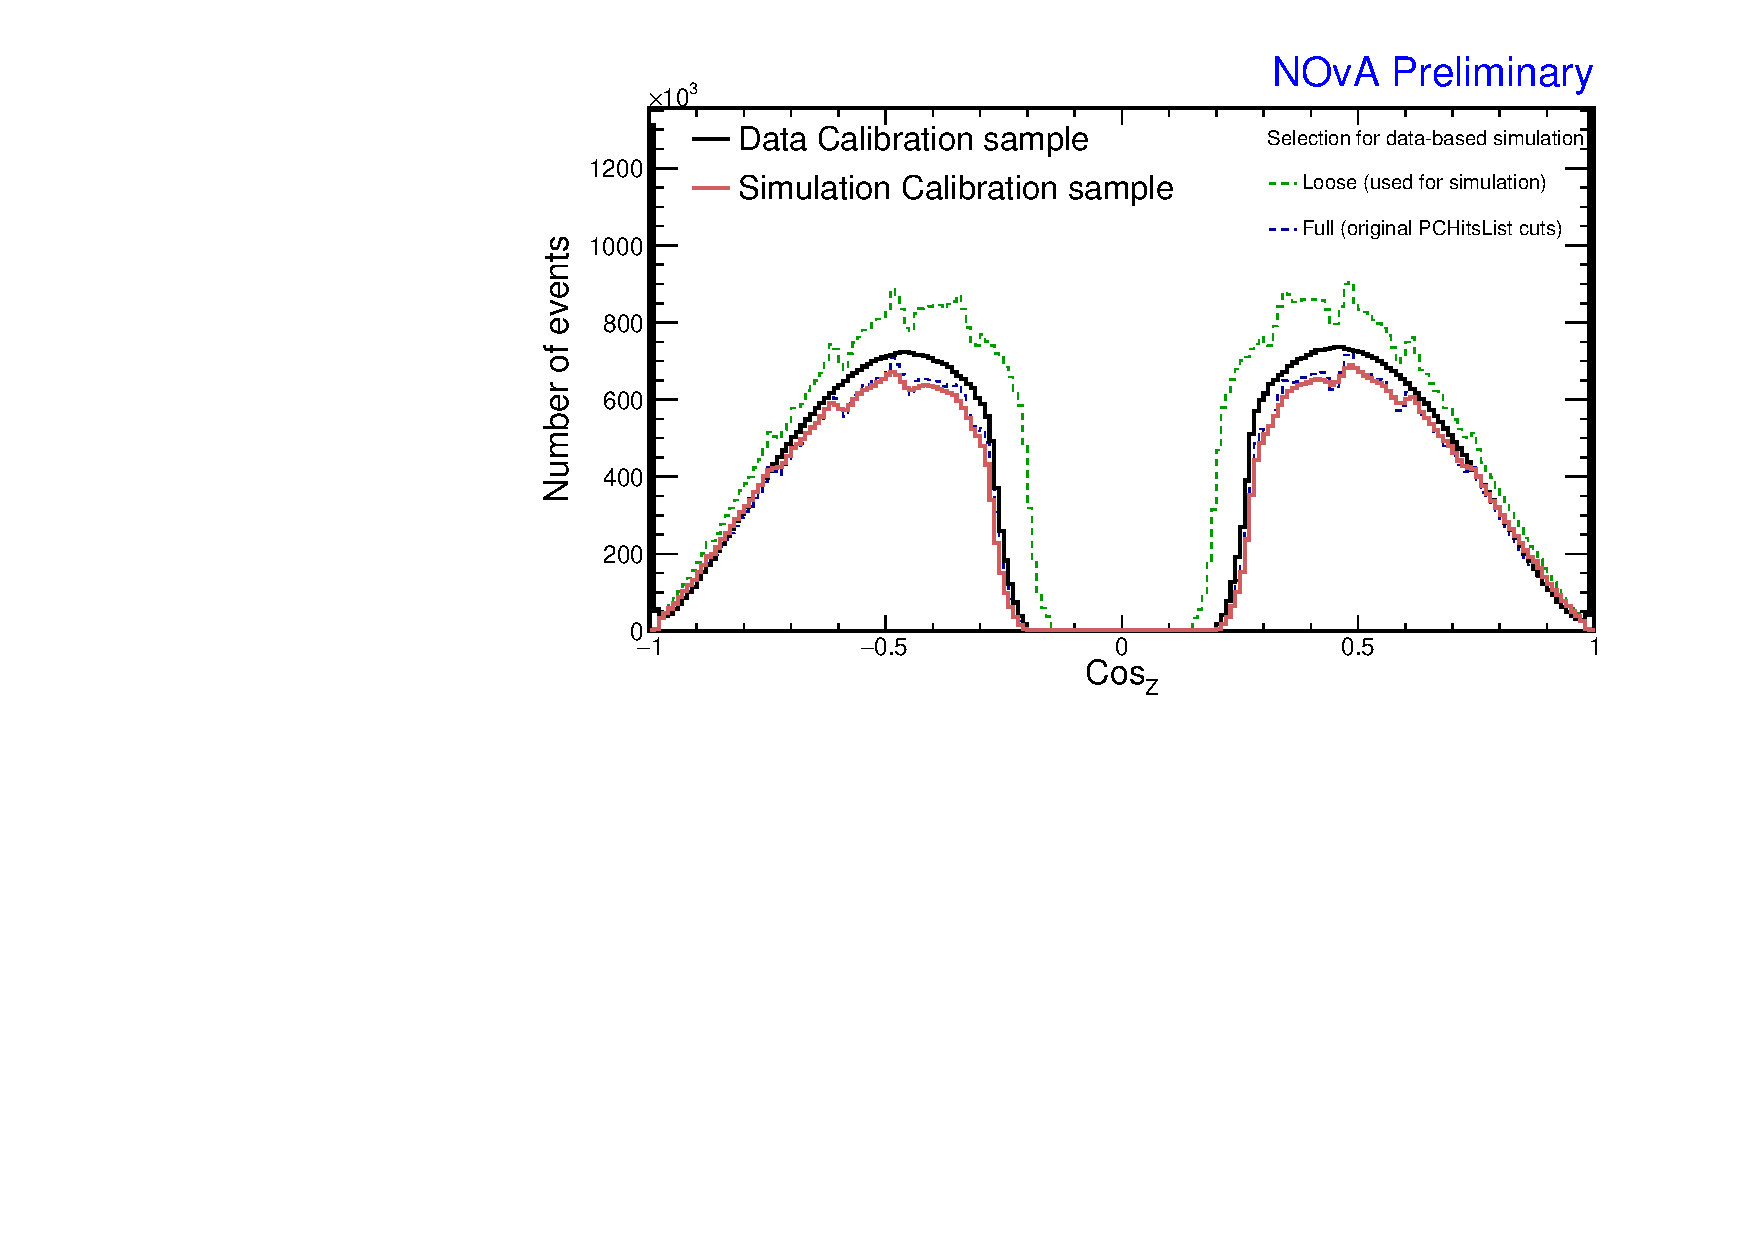
\includegraphics[width=\textwidth]{Plots/TBCalibration/DBSim_DataMCComparison_CosZ.pdf}
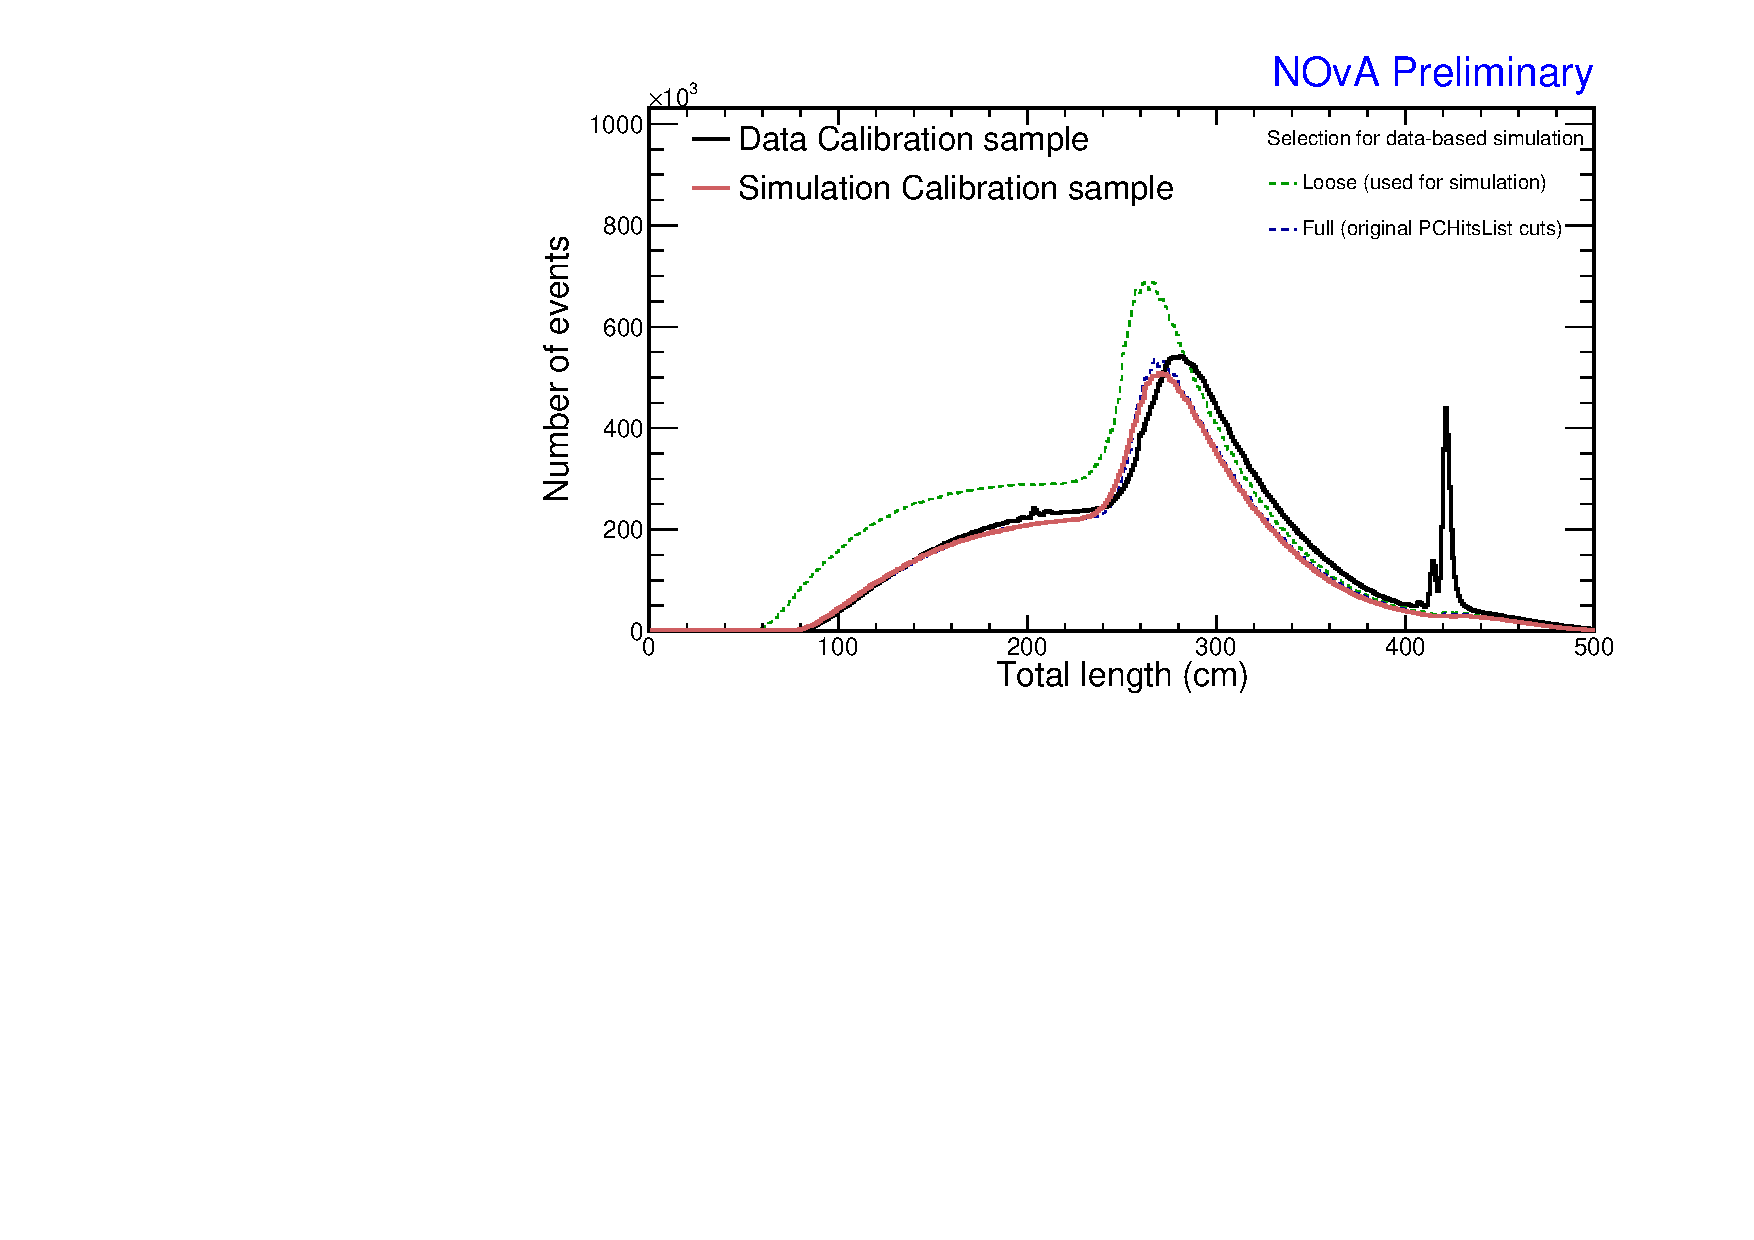
\includegraphics[width=\textwidth]{Plots/TBCalibration/DBSim_DataMCComparison_TotLength.pdf}
\caption[Data-Simulation comparison of angular and track length distributions]{Comparison of the angle from the z axis and total track length between the data (black) and simulation (pink) calibration samples, as detailed in the text. Additionally, the distributions of data with full (blue) and loose (green) selections applied to the \acrshort{BPF} tracks are shown, where the loose selection was used to create the simulation.}
\label{fig:DataBasedSimDataMCComparison_cosZtotLength}
\end{figure}

\begin{figure}[!ht]
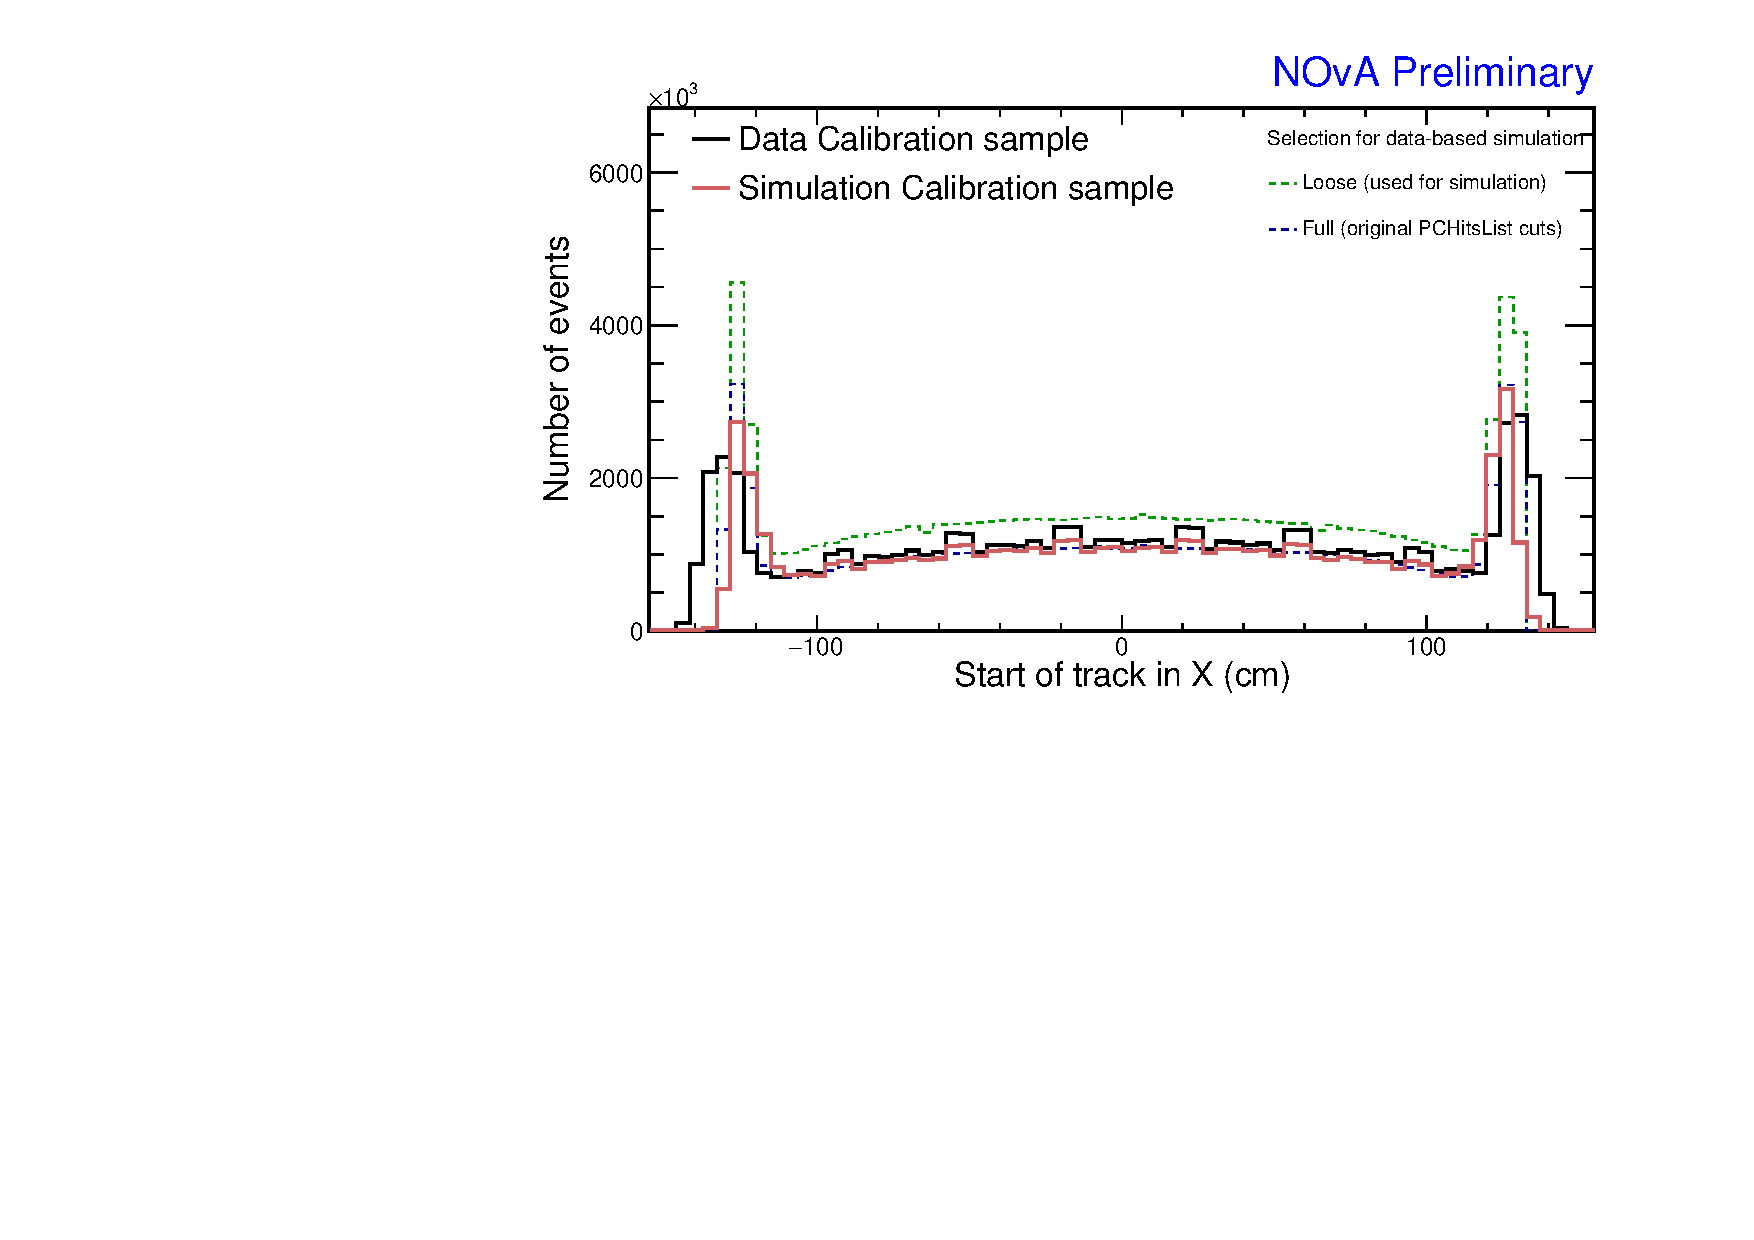
\includegraphics[width=\textwidth]{Plots/TBCalibration/DBSim_DataMCComparison_StartX.pdf}
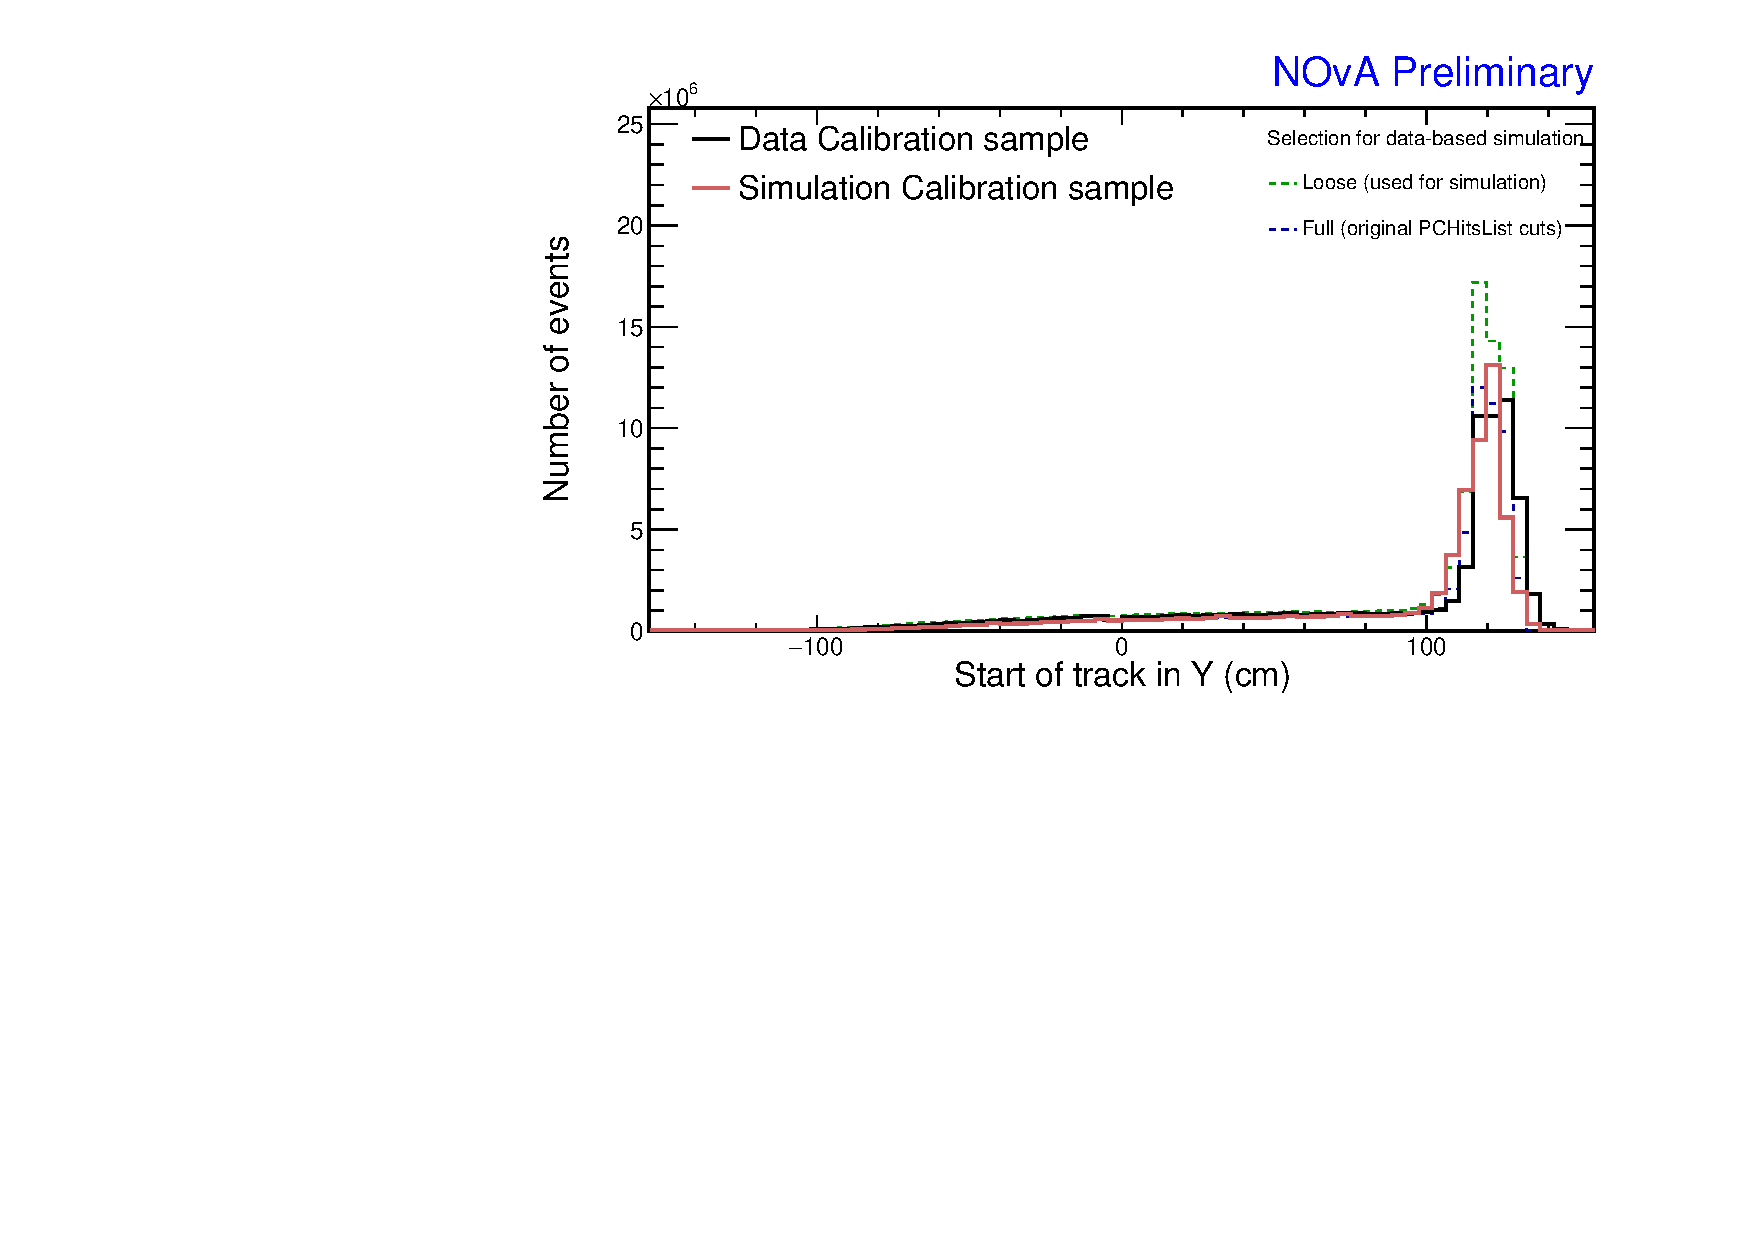
\includegraphics[width=\textwidth]{Plots/TBCalibration/DBSim_DataMCComparison_StartY.pdf}
\caption[Data-Simulation comparison of track start X and Y distributions]{Comparison of the x (top) and y (bottom) track start position between the data (black) and simulation (pink) calibration samples, as detailed in the text. Additionally, the distributions of data with full (blue) and loose (green) selections applied to the \acrshort{BPF} tracks are shown, where the loose selection was used to create the simulation.}
\label{fig:DataBasedSimDataMCComparison_startXstartY}
\end{figure}

\begin{figure}[!ht]
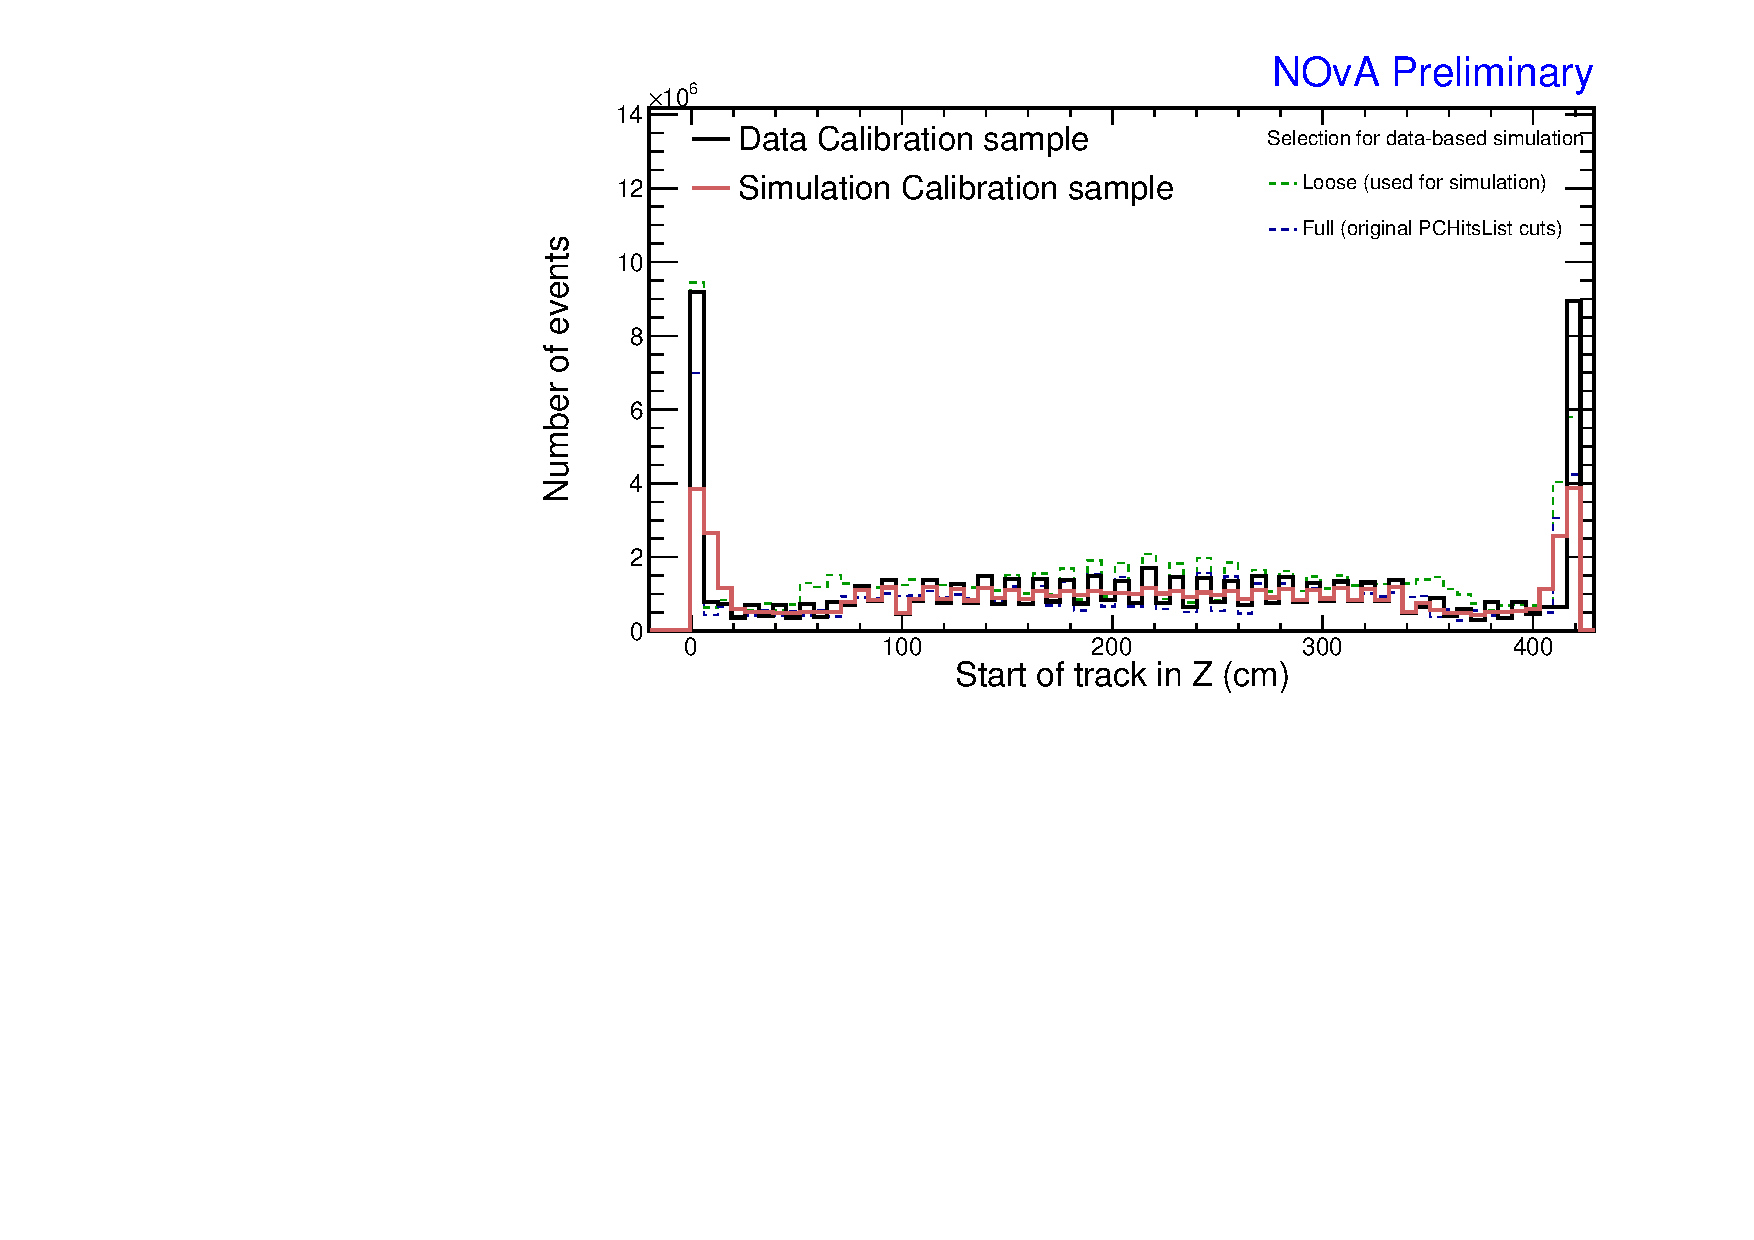
\includegraphics[clip, width=\textwidth]{Plots/TBCalibration/DBSim_DataMCComparison_StartZ.pdf}
\caption[Data-Simulation comparison of track start Z distribution]{Comparison of the z track start position between the data (black) and simulation (pink) calibration samples, as detailed in the text. Additionally, the distributions of data with full (blue) and loose (green) selections applied to the \acrshort{BPF} tracks are shown, where the loose selection was used to create the simulation. Each bin corresponds to a single detector plane and the shape of the distribution is caused by the fact that cosmic rays are naturally more vertical and therefore more likely to be detected by horizontal than vertical planes.}
\label{fig:DataBasedSimDataMCComparison_startZ}
\end{figure}

%%% Simulation is like the full calibration cuts applied to BPF cuts
It can be seen that the distributions of the new simulation calibration sample resemble those of the data \gls{BPF} tracks with full calibration cuts applied (blue dashed lines) more closely than those of the data calibration sample. This indicates that the simulated window cosmic tracks have similar properties to the data \gls{BPF} tracks, meaning that the differences between the tracking algorithms have an impact on the resulting simulation. Therefore, loosening the calibration cuts did not help with mitigating these differences as expected. However, there were in total four versions of simulation created, with varying event selections and smearing applied, including using full calibration cuts and with different loosened calibration cut values. It is clear that it is unlikely we can mitigate the differences between the window cosmic tracks and the \gls{BPF} tracks simply by changing the event selection or smearing and it would require adapting (or developing) a different reconstruction algorithm for the simulation. Due to the time and effort required for such a task, and due to the relative similarity between the simulation and data calibration samples, we decided to proceed with the reconstruction, selection, and correction as described above.

%%% Beam-like data removed (refer back to selection)
Figures~\ref{fig:DataBasedSimDataMCComparison_cosXcosY} and \ref{fig:DataBasedSimDataMCComparison_cosZtotLength} show the effect of removing the beam-like events with a $\left|\textsf{Cos}_Z\right|<0.98$ cut as described in Sec.~\ref{sec:DataBasedSimSelection}.  While we applied this cut to the data events used to create the simulation (green dashed lines), it is not included in the selection process for the calibration samples. This means that we were successful in removing these undesirable events from the new simulation. This can be seen by the wide peaks at $\textsf{Cos}_{X/Y}=0$ in Fig.~\ref{fig:DataBasedSimDataMCComparison_cosXcosY} which are present for the data calibration sample, by not for the simulation. Additionally, sharp peaks in the total track length and in the edges of the angle from the z axis distributions in Fig.~\ref{fig:DataBasedSimDataMCComparison_cosZtotLength} further illustrate this distinction.
%The wide peaks at $\textsf{Cos}_{X/Y}=0$ correspond to tracks parallel to the z axis, which are likely leftover beam events that were removed for simulation (Sec.~\ref{sec:DataBasedSimSelection}, but not in data.
%The simulation calibration sample has an additional cut on $\left|\textsf{Cos}_Z\right|<0.98$ that removes beam-like events (Sec.~\ref{sec:DataBasedSimSelection}) compared to data. This can be clearly seen on the top plot with peaks on the left and right sides if the data calibration sample's distribution, which are removed for in simulation. It can also be seen in the bottom plot, where the removed beam-like events correspond to the peaks around $\unit[200]{cm}$ and $\unit[420]{cm}$.

%%% Rugged shape helped a little by smearing
The effect of smearing of vertex positions and four momenta is visible in the top plot of Fig.~\ref{fig:DataBasedSimDataMCComparison_cosZtotLength} and in Fig.~\ref{fig:DataBasedSimDataMCComparison_startZ}. Here, the ridged distributions of the data used for simulation (green dashed lines) appears smoother for the simulation calibration sample (pink solid lines). However, comparisons of track start positions in Fig.~\ref{fig:DataBasedSimDataMCComparison_startXstartY} and \ref{fig:DataBasedSimDataMCComparison_startZ} show that the simulated events start further away from the detector edge compared to data. While this is likely also a result of smearing, we anticipate it will not impact the calibration of the simulated detector.
% The simulation calibration sample has a smaller differences between the horizontal and vertical planes, presumably due to the smearing applied (Sec~\ref{sec:DataBasedSimPython}).

%%% Smearing (or reco?) caused events to start more inside of the detector
%The start of track comparison between data and simulation in Fig.~\ref{fig:DataBasedSimDataMCComparison_startXstartY} and \ref{fig:DataBasedSimDataMCComparison_startZ} show that there are fewer events that start at the edge of the detector and the vertex positions are moved slightly towards the inside of the detector. This is likely the result of the smearing of the vertex positions and we do not expect this to have an effect on the calibration. 

%%% Adding re-simulation samples
After adding the distributions for the re-simulation calibration sample, shown as solid brown lines Fig.~\ref{fig:DataBasedSimSimVersionComparison}, we can see that the track start positions are shifted even further towards the inside of the detector. This would support the hypothesis that this effect is caused by smearing and is also likely related to the loss of events with longer track lengths, as shown in Fig.~\ref{fig:DataBasedSimSimVersionComparison}, since if tracks start a few centimetres later in the detector their tracks would get shorter by the same amount. Since there are only minimal discrepancies between the simulation and the re-simulation, we conclude that the reconstruction, selection and correction processes used to create the simulation do not significantly bias the simulation, which is self-consistent.

\begin{figure}[!ht]
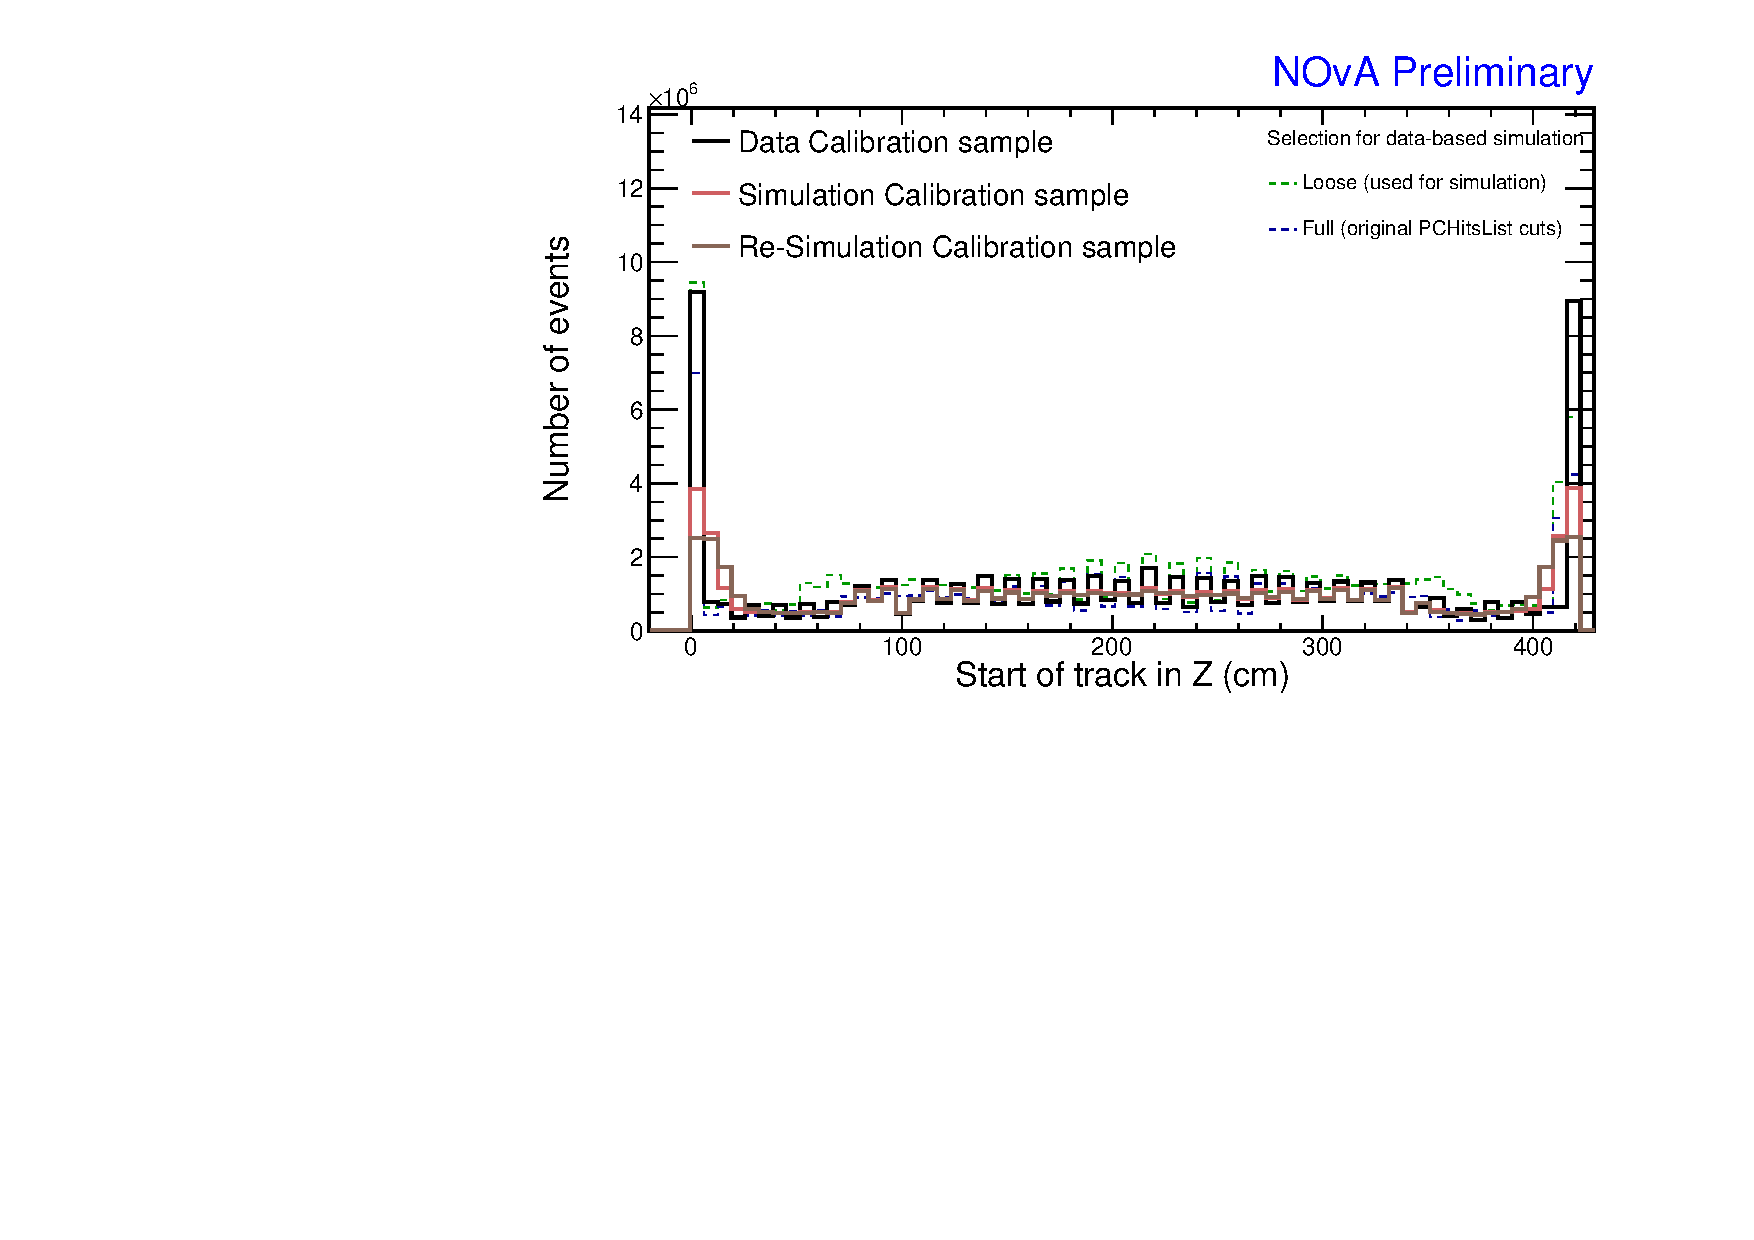
\includegraphics[width=\textwidth]{Plots/TBCalibration/DBSim_SimVersionComparison_StartZ.pdf}
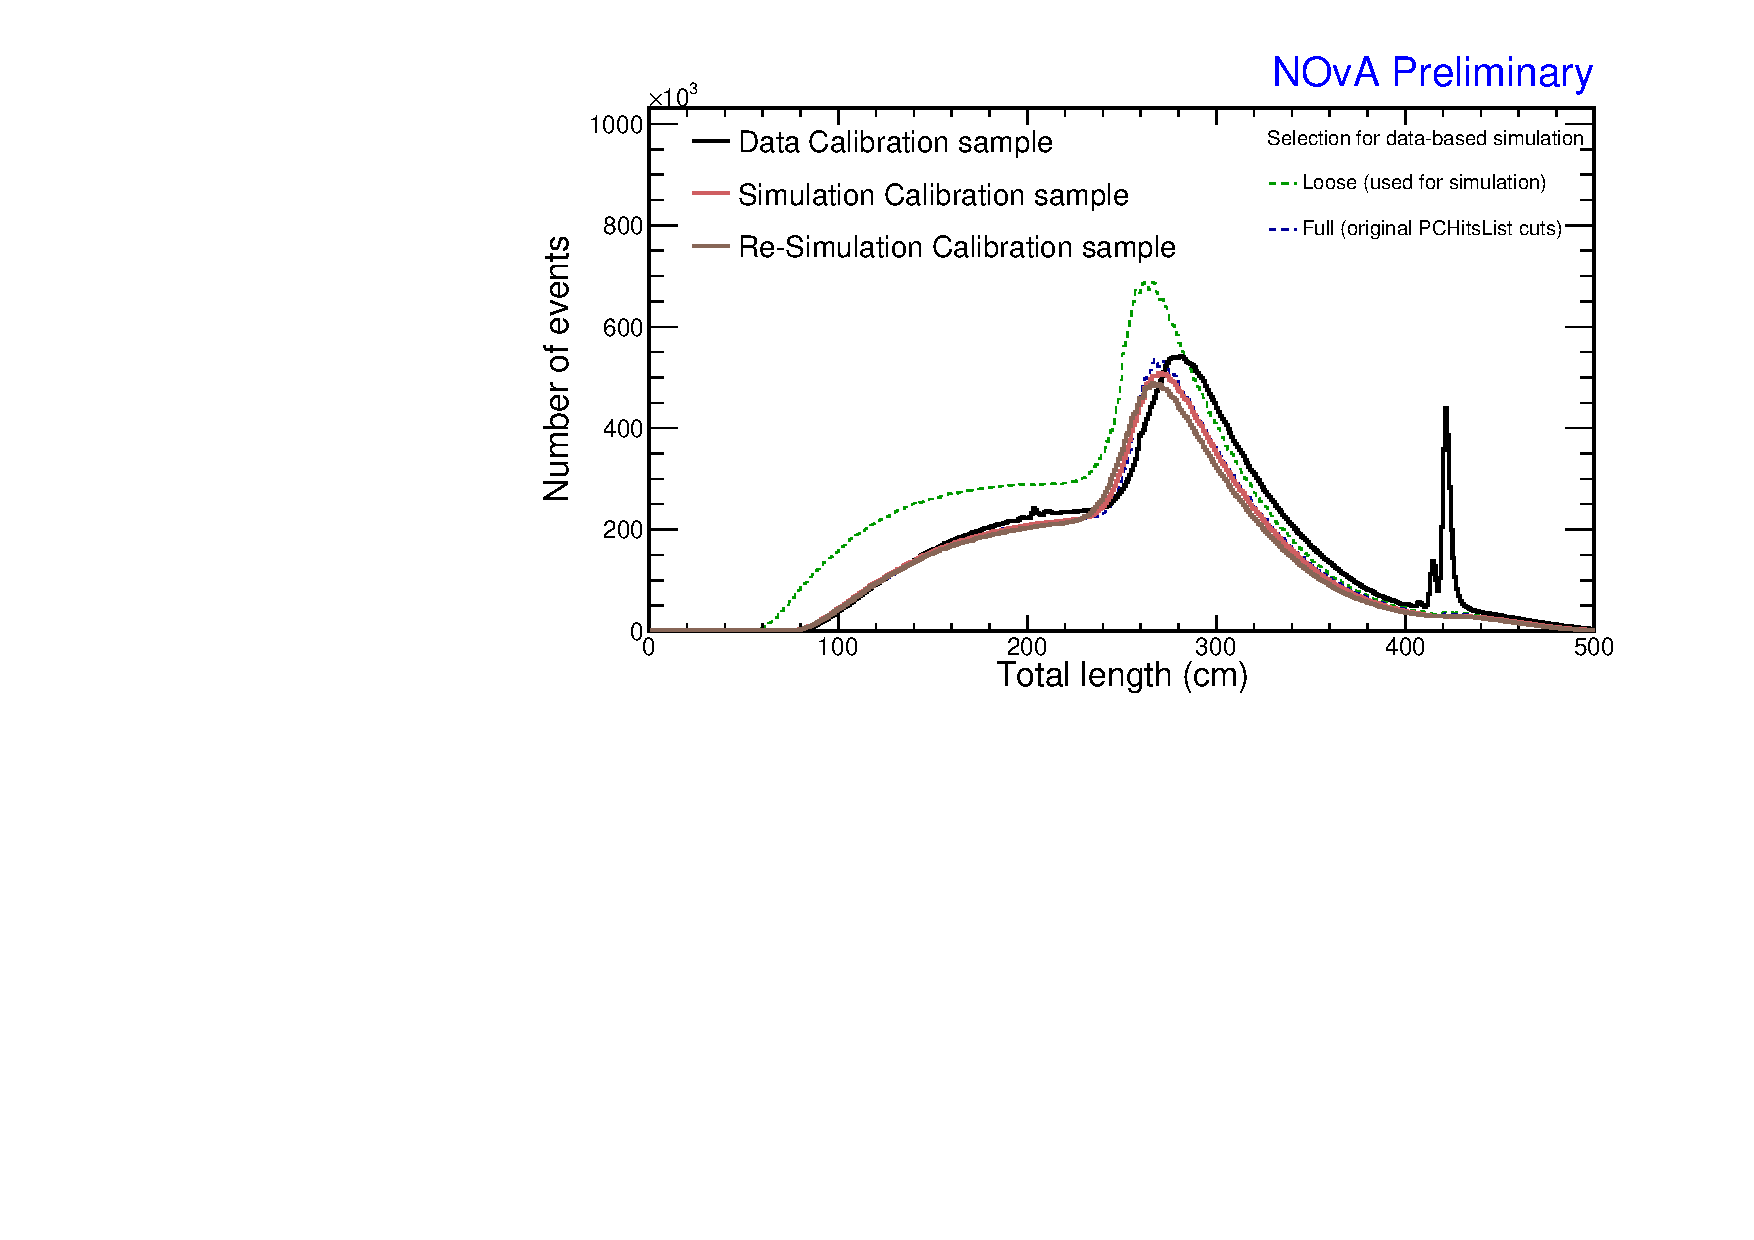
\includegraphics[width=\textwidth]{Plots/TBCalibration/DBSim_SimVersionComparison_TotLength.pdf}
\caption[Comparison of simulation to a re-simulation validation sample]{Comparison of the z track start position and total track length between the re-simulated events (brown), which use simulation as `fake data' for the second iteration of the same simulation process, and the data (black) and simulation (pink) events. Additionally, the distributions of data with full (blue) and loose (green) selections applied to the \acrshort{BPF} tracks are shown, where the loose selection was used to create the simulation.}
\label{fig:DataBasedSimSimVersionComparison}
\end{figure}

\section{Summary}\label{sec:DataBasedSimSummary}
I have successfully developed a new simulation of cosmic muons intended for Test Beam calibration. The reconstruction, selection, and correction processes were designed to minimize the number of simulated events, resulting in an efficient and concise simulation while avoiding a significant bias, particularly in the applicability to the calibration procedures.

While the simulation achieved its objectives, there are possible improvements that could be introduced to refine it. Using a different track reconstruction algorithm than the \gls{BPF}, more consistent with the window cosmic track algorithm, could make the simulation calibration sample more alike the data calibration sample. Additionally, developing a more sophisticated energy correction procedure, potentially involving external measurements of energy distribution of cosmic muons, would enable simulation of through-going muons with accurate incident energies.

Looking ahead, there are plans to use the data-based simulation approach for cosmic muons in the \gls{NOvA} \gls{ND} and \gls{FD}. While the primary motivation is again detector calibration, there is potential for broader applications in cosmic ray studies. However, using the simulation for a different detector would require re-validating the event selection process, especially with the inclusion of the calibration cuts missing for the Test Beam detector, as outline in Sec.~\ref{sec:DataBasedSimSelection} and showed shaded out in two bottom rows of Tab.~\ref{tab:DataBasedSimEventSelection}.